% TEX root = ../main.tex
\chapter{Algoritmi deterministici}

Come anticipato, in questo corso tratteremo inizialmente gli algoritmi deterministici.

\section{Problema del matching bipartito massimale}
% disegno grafo bipartito: nove vertici, cinque a sinistra e quattro a destra, 
% 1l, 2l, 4l, 5l -> 1d; 3l -> 2d, 3d; 4l ->4d.
\popt {BipartiteMaxMatching} {$G = (V,E)$ \textit{bipartito}} {Insieme di lati}
{Qual è il \textit{matching} più ampio?} {Scelte di insiemi di lati che siano \textit{matching}}
{$Max$}{Cardinalità dell'insieme}

\noindent
Un grafo \textit{bipartito} è un grafo non orientato in cui l'insieme dei vertici
è diviso in due parti; tutti i lati hanno un'estremità che incide su una parte
e un'estremità che incide sull'altra, come rappresentato nella figura \ref{fig:graphmatching}.

\begin{figure}[h]
	\centering
	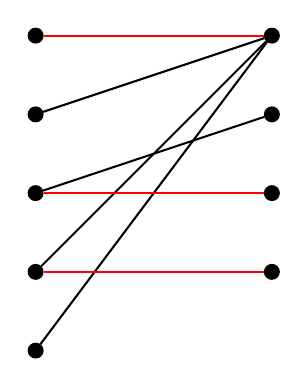
\begin{tikzpicture}

		\node[draw,inner sep=0pt,minimum size=5pt,fill, circle] at (0, 1)  (a) {};
		\node[draw,inner sep=0pt,minimum size=5pt,fill, circle] at (0, 2)  (b) {};
		\node[draw,inner sep=0pt,minimum size=5pt,fill, circle] at (0, 3)  (c) {};
		\node[draw,inner sep=0pt,minimum size=5pt,fill, circle] at (0, 4)  (d) {};
		\node[draw,inner sep=0pt,minimum size=5pt,fill, circle] at (0, 5)  (e) {};

		\node[draw,inner sep=0pt,minimum size=5pt,fill, circle] at (3, 2)  (f) {};
		\node[draw,inner sep=0pt,minimum size=5pt,fill, circle] at (3, 3)  (g) {};
		\node[draw,inner sep=0pt,minimum size=5pt,fill, circle] at (3, 4)  (h) {};
		\node[draw,inner sep=0pt,minimum size=5pt,fill, circle] at (3, 5)  (i) {};

		\draw (a) -- (i);
		\draw (b) -- (i);
		\draw (d) -- (i);
		\draw[red] (e) -- (i);
		\draw[red] (b) -- (f);
		\draw[red] (c) -- (g);
		\draw (c) -- (h);
	\end{tikzpicture}
	\caption{Esempio di un grafo bipartito. I lati colorati rappresentano un possibile \textit{matching}.}
	\label{fig:graphmatching}
\end{figure}

Le soluzioni ammissibili sono dei \textit{matching}, ossia una scelta di lati
tale che nessun vertice abbia più di un lato incidente. L'obiettivo è trovare il
matching più grande possibile, ossia quello col numero maggiore di lati.
La funzione di costo è quindi la cardinalità dell'insieme di matching,
e il problema è di massimo.

Questo problema si può risolvere polinomialmente. Esiste anche un algoritmo
che risolve questo problema anche sui grafi generali, ma sono molto complessi.

% lezione 3 - 06/10/2021
\subsection{Algoritmo basato su cammini aumentanti}
Dato un grafo $G$ e un matching $M$ possiamo definire \textit{occupati}
i lati presenti nel matching. Un vertice \textit{esposto} è un vertice su
cui non incidono lati occupati. Nei vertici non esposti può incidere al massimo
uno ed un solo lato occupato (altrimenti non sarebbe un matching). A partire
da questa definizione, possiamo definire i \textbf{cammini aumentanti}:
essi sono cammini che alternano lati liberi e lati occupati, iniziando e
terminando su un vertice esposto.

Dato il cammino aumentante, possiamo rimuovere dal matching tutti i lati
\textit{occupati} dal cammino aumentante e possiamo inserivi tutti i lati che non
erano presenti. Questa operazione si chiama \textbf{switch del cammino aumentante}:
alcuni lati sono stati inseriti, altri sono stati rimossi. Il matching risultante
può essere più grande o più piccolo, ma dovremo comunque controllare se effettivamente
ciò che risulta è un matching.

%disegno: inversione selezione cammini del disegno precedente

\begin{figure}[h]
	\centering
	\begin{subfigure}[b]{0.4\textwidth}
		\centering
		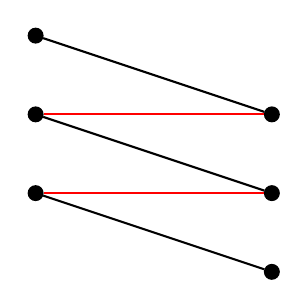
\begin{tikzpicture}

			\node[draw,inner sep=0pt,minimum size=5pt,fill, circle] at (3, 1)  (a) {};
			\node[draw,inner sep=0pt,minimum size=5pt,fill, circle] at (0, 2)  (b) {};
			\node[draw,inner sep=0pt,minimum size=5pt,fill, circle] at (0, 3)  (c) {};
			\node[draw,inner sep=0pt,minimum size=5pt,fill, circle] at (3, 2)  (f) {};
			\node[draw,inner sep=0pt,minimum size=5pt,fill, circle] at (3, 3)  (g) {};
			\node[draw,inner sep=0pt,minimum size=5pt,fill, circle] at (0, 4)  (h) {};

			\draw (a) -- (b);
			\draw[red] (b) -- (f);
			\draw (f) -- (c);
			\draw[red] (c) -- (g);
			\draw (g) -- (h);

		\end{tikzpicture}
		\subcaption{Prima dello switch.}
	\end{subfigure}
	\begin{subfigure}[b]{0.4\textwidth}
		\centering
		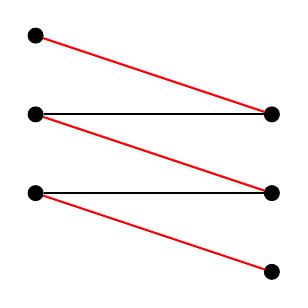
\begin{tikzpicture}

			\node[draw,inner sep=0pt,minimum size=5pt,fill, circle] at (3, 1)  (a) {};
			\node[draw,inner sep=0pt,minimum size=5pt,fill, circle] at (0, 2)  (b) {};
			\node[draw,inner sep=0pt,minimum size=5pt,fill, circle] at (0, 3)  (c) {};
			\node[draw,inner sep=0pt,minimum size=5pt,fill, circle] at (3, 2)  (f) {};
			\node[draw,inner sep=0pt,minimum size=5pt,fill, circle] at (3, 3)  (g) {};
			\node[draw,inner sep=0pt,minimum size=5pt,fill, circle] at (0, 4)  (h) {};

			\draw[red] (a) -- (b);
			\draw (b) -- (f);
			\draw[red] (f) -- (c);
			\draw (c) -- (g);
			\draw[red] (g) -- (h);

		\end{tikzpicture}
		\subcaption{Dopo lo switch.}
	\end{subfigure}
	\caption{Esempio di un cammino aumentante in un grafo bipartito. I lati colorati rappresentano i lati selezionati nel matching.}
	\label{fig:augpaths}
\end{figure}

\begin{theorem}
	Esiste un cammino aumentante per $M$ se e solo se $M$ non è massimo.
\end{theorem}
\begin{proof}

	\begin{itemize}
		\item[$\implies$] banale dall'operazione di switch.

		\item[$\impliedby$] Ipotizziamo, per assurdo, che $M$ non sia massimo
			e non esistano cammini aumentanti. Sia $M'$ un matching tale che $|M'| > |M|$.
			Sia $X = M\Delta M' = (M \setminus M') \cup (M' \setminus M)$.

			Su ogni vertice incidono al massimo due lati di $X$, ossia
			in $X$ vi saranno alcuni vertici con grado $0$, $1$ oppure $2$
			(se ci fossero con grado $3$, allora uno dei due matching non sarebbe
			davvero un matching).

			Se si trova un ciclo in $X$ con un lato in $M \setminus M'$, quello seguente
			dovrà essere in $M' \setminus M$, quello seguente ancora sarà in $M \setminus M'$
			e così via; i cicli hanno pertanto per forza lunghezza pari.
			Ogni ciclo, quindi, ``cancella'' una quantità uguali di lati dalle due metà
			($M \setminus M'$, $M' \setminus M$).

			Ma deve essere per forza $|M' \setminus M| > |M \setminus M'|$,  poiché
			$M'$ è un matching più ampio di $M$. Oltre ai cicli si devono considerare
			anche i cammini: vi deve essere un cammino in $X$ che ha più lati in $M' \setminus M$:
			i lati saranno alternati, nuovamente, tra lati in $M\setminus M'$ e lati in
			$M' \setminus M$: i vertici estremi devono essere esposti in $M$,
			altrimenti ci sarebbe un lato di $M$ che incide su di esso, che però non può stare in $M'$.
			Pertanto, questo cammino è un cammino aumentante per $M$.
	\end{itemize}
\end{proof}

\noindent
L'algoritmo è definito come segue.

\begin{algorithm}[!ht]
	\caption{\textsc{BipartiteMaxMatching}}
	\KwInput{grafo $G = (V,E)$}
	\KwOutput{Matching massimale per $G$}

	$ M = \emptyset $

	\While{$\exists \text{ cammino aumentante } \pi \text{ per } M $}
	{
		esegui uno switch su $\pi$
	}
\end{algorithm}

Dimostriamo ora che se $G$ è bipartito, calcolare se esiste un cammino
aumentante ha costo $O(nm)$, rendendo la complessità in tempo
$$
	O(n^2m)
$$

Dimostrare che esiste un cammino aumentante esiste richiede una visita;
procediamo, quindi, con un breve intermezzo riguardo la visita dei grafi.

\subsubsection{Visite di grafi}
Le visite dei grafi (\textit{graph traversal}) sono algoritmi nei quali i vertici
del grafo, in ogni istante, possono rientrare in tre categorie:
\begin{itemize}
	\item{\bf bianchi}: sono vertici sconosciuti e non esplorati.
	\item{\bf grigi}: sono vertici conosciuti ma non esplorati. Vengono anche
	chiamati \textit{nodi di frontiera}. Essi sono contenuti in un'apposita
	struttura dati chiamata \textit{dispenser}, che effettivamente classifica
	la visita.
	\item{\bf neri}: sono vertici conosciuti e visitati.
\end{itemize}

L'algoritmo generale di visita è l'algoritmo \ref{algo:genericgraphvisit}.

\begin{algorithm}[h]
	\caption{\textsc{GenericGraphVisit}}
	\label{algo:genericgraphvisit}
	\KwInput{grafo $G = (V,E)$, vertice $v_0$}
	\For {$v \in V(G)$}
	{
		$v.color = bianco$
	}
	$ F = v_0$ \tcc* {$F$ è un \textit{dispenser} di vertici, e.g. stack}
	$ v_0.color = grigio$

	\While{!F.empty()}
	{
		v = F.get()

		visit(v)

		\tcc*{$N(v)$ estrae i successori di $v$}
		\For {w : N(v)}
		{

			\If{w.color = bianco}
			{

				F.insert(w)

				w.color = grigio

			}
		}
		v.color = nero
	}
\end{algorithm}

La visita dipende dalla struttura $F$: se $F$ è una coda, la visita sarà in
ampiezza, mentre se è uno stack la visita sarà in profondità. Chiaramente,
non è detto che al termine dell'algoritmo tutti i vertici siano stati visitati,
infatti, se non esiste un cammino tra il nodo seme ed un altro nodo,
quest'ultimo non sarà mai visitato (pertanto, le visite possono essere utilizzate
anche per trovare le componenti connesse.)
Ogni visita richiede tempo $O(m)$,  poiché di tutti i nodi si guardano i vicini una volta sola.

\noindent
\newline
Un cammino aumentante è un cammino che comincia e termina in un vertice esposto e
alterna lati nel matching a lati esterni. Inizialmente, possiamo limitarci
a cercare tali cammini tra quelli che partono da un vertice esposto;
eseguiamo quindi una visita in ampiezza (ossia $F$ è una coda) alternando i lati
liberi ai lati occupati. Se nel corso della visita si trova un vertice
esposto. Questo algoritmo funziona solo su grafi
bipartiti: si supponga di cominciare la visita dal nodo $6$ in figura \ref{fig:augmentingvisit}.
I vicini di $6$ sono $2$ e $5$: supponiamo di scegliere il lato $6 \rightarrow 2$.
I vicini di $2$ sono $3$ e $1$. Selezioniamo l'unico lato coperto,
$2 \rightarrow 3$. I vicini di $3$ sono $4$ e $2$ (che è nero);
selezioniamo l'unico lato non coperto, $3 \rightarrow 4$.
Procediamo con $4\rightarrow 5$. La visita termina.
Il cammino aumentante esiste:
$6 \rightarrow 5 \rightarrow 4 \rightarrow 3 \rightarrow 2 \rightarrow 1$.

\begin{figure}[h]
	\centering
	\begin{subfigure}[b]{0.4\textwidth}
		\centering
		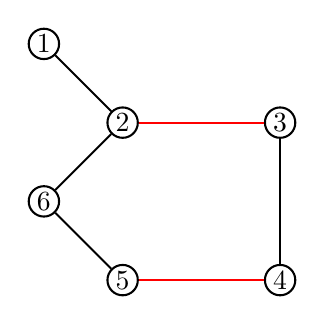
\begin{tikzpicture}
			\node[draw,inner sep=1pt,minimum size=8pt, circle] at (0, 3)  (1) {1};
			\node[draw,inner sep=1pt,minimum size=8pt, circle] at (1, 2)  (2) {2};
			\node[draw,inner sep=1pt,minimum size=8pt, circle] at (3, 2)  (3) {3};
			\node[draw,inner sep=1pt,minimum size=8pt, circle] at (3, 0)  (4) {4};
			\node[draw,inner sep=1pt,minimum size=8pt, circle] at (1, 0)  (5) {5};
			\node[draw,inner sep=1pt,minimum size=8pt, circle] at (0, 1)  (6) {6};

			\draw (1) -- (2);
			\draw[red] (2) -- (3);
			\draw (2) -- (6);
			\draw (6) -- (5);
			\draw (3) -- (4);
			\draw[red] (5) -- (4);

		\end{tikzpicture}
		\subcaption{Situazione ipotetica in cui solo due lati, quelli rossi, sono
			inseriti nel matching.}
	\end{subfigure}
	\begin{subfigure}[b]{0.4\textwidth}
		\centering
		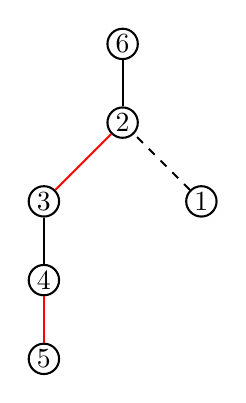
\begin{tikzpicture}
			\node[draw,inner sep=1pt,minimum size=8pt, circle] at (1, 4) (6) {6};
			\node[draw,inner sep=1pt,minimum size=8pt, circle] at (1, 3) (2) {2};
			\node[draw,inner sep=1pt,minimum size=8pt, circle] at (0, 2) (3) {3};
			\node[draw,inner sep=1pt,minimum size=8pt, circle] at (2, 2) (1) {1};
			\node[draw,inner sep=1pt,minimum size=8pt, circle] at (0, 1) (4) {4};
			\node[draw,inner sep=1pt,minimum size=8pt, circle] at (0, 0) (5) {5};

			\draw[dashed] (1) -- (2);
			\draw[red] (2) -- (3);
			\draw (2) -- (6);
			\draw (3) -- (4);
			\draw[red] (5) -- (4);

		\end{tikzpicture}
		\subcaption{Visita per la creazione del cammino aumentante a partire dal nodo $6$.}
	\end{subfigure}

	\caption{Esemplificazione dell'algoritmo per trovare cammini aumentanti.}
	\label{fig:augmentingvisit}
\end{figure}
\begin{theorem}
	\textsc{BipartiteMaxMatching} $\in \mathbf{PO}$.
\end{theorem}

\begin{corollario}
	Il problema del \textsc{PerfectMatching}
	(dato un grafo, decidere se esiste un matching
	che incide su tutti i vertici) è in $\mathbf{P}$.
\end{corollario}
Questo deriva dal fatto
che se esiste un matching perfetto per un grafo, il matching massimo avrà cardinalità $n/2$.

\noindent
Tutti gli altri problemi che vedremo saranno in $\mathbf{NPO-completi}$.
\vfill

\section{Problema del bilanciamento del carico}
\popt {LoadBalancing} {$n$ task $t_0, t_1, \cdots, t_{n-1} \in \mathbb{N}^+$, $m$ macchine}
{Insieme di assegnamenti di task a macchine}
{Qual è l'assegnamento con costo massimo minore?}
{Scelte di assegnamenti di tutti i task alle macchine in modo coerente}
{$Min$}
{Ogni macchina ha carico $L_i = \sum_{j \text{ assegnato a } i } t_j$
    la funzione obiettivo è $L=\max_i L_i$}
Per esempio, si supponga di avere $8$ task e $3$ macchine. I task hanno costo
$\{3, 2, 3, 1, 1, 4, 5, 1\}$; vi sono diversi modi per assegnare le task:
\begin{itemize}
	\item{$m_0$}: $\{5, 1,1\}$ con $L_0 = 7$
	\item{$m_1$}: $\{4, 3\}$ con $L_1 = 7$
	\item{$m_2$}: $\{2, 3, 1\}$ con $L_2 = 6$.
\end{itemize}
Pertanto $L = 7$.

\begin{theorem}
	\textsc{LoadBalancing} $ \in \mathbf{NPO-completi}$.
\end{theorem}

\subsection{Algoritmo greedy balance}
Un algoritmo banale per risolvere approssimativamente il problema \textsc{LoadBalancing} è
l'algoritmo \ref{algo:greedybalance}.

\begin{algorithm}[!ht]
	\caption{\textsc{GreedyBalance}}
	\label{algo:greedybalance}
	\KwInput{$m$ macchine, $n$ task con costi $t_i$}

	\For{$i$ : $0..n-1$}
	{
		$L_i = 0$
	}

	\For{$j$ : $0..n-1$}
	{
		$ \bar{i} = \arg \min (L_i)$

		$M_i.addTask(t_j)$

		$L_i = L_i + t_j$
	}

\end{algorithm}
\noindent
Questo algoritmo ha complessità $O(n \log(n))$.

\begin{theorem} \label{thm:gbal_2_approx}
	\textsc{GreedyBalance} è un algoritmo $2$-approssimante per \textsc{LoadBalancing}.
\end{theorem}

\noindent
Prima di procedere con la dimostrazione, sono necessarie due osservazioni:

\begin{lemma}
	\label{lem:gbal_opt_gt_frac_sum}
	$$
		L^* \geq \frac{1}{m} ~ \sum_j t_j
	$$
\end{lemma}
\begin{proof}
	Si supponga di avere la soluzione ottima. Si ha che
	$$
		\sum_{i = 0}^{m-1} L^*_i = \sum_{j = 0}^{n-1} t_j
	$$
	e pertanto
	$$
		L^* = \max\{L^*_i\}_i \geq \frac{1}{m} \sum_j t_i
	$$
\end{proof}

\begin{lemma}
	\label{lem:gbal_opt_gt_max}
	$$
		L^* \geq \max_j t_j
	$$
\end{lemma}
\begin{proof}
	Banale.
\end{proof}

Passiamo alla dimostrazione del \cref{thm:gbal_2_approx}.
\begin{proof}
	Eseguiamo \textsc{GreedyBalance}; sia $\hat{i}$ la macchina più carica al termine
	dell'esecuzione, ossia $L = L_{\hat{i}}$. Sia $\hat{j}$ l'ultimo task assignato
	alla macchina $\hat{i}$. Prima di ricevere $\hat{j}$, il suo carico è tale per cui
	$$
		\forall i = 1..m ~ L_{\hat{i}} - t_{\hat{j}} \leq L'_i \leq L_i
	$$
	dove $L'_{i}$ è il carico della macchina $i$ quando il task $\hat{j}$ è
	deve essere assegnato. Sommiamo quindi su tutti gli $i$:
	$$
		m \cdot (L_{\hat{i}} - t_{\hat{i}}) \leq \sum_{i = 1}^{m} L_i = \sum_{j = 0}^{n-1} t_j
	$$
	poiché tutte le task sono state assegnate. Grazie al \cref{lem:gbal_opt_gt_frac_sum}
	possiamo affermare
	$$
		L_{\hat{i}} - t_{\hat{i}} \leq \frac{1}{m} \sum_i L_i \leq L^*
	$$
	\`E ovvio che $L = L_{\hat{i}} = (L_{\hat{i}} - t_{\hat{j}}) + t_{\hat{j}}$ e
	sappiamo anche che $t_{\hat{j}} \leq L^*$ dal \cref{lem:gbal_opt_gt_max};
	possiamo quindi concludere
	$$
		L = (L_{\hat{i}} - t_{\hat{j}}) + t_{\hat{j}} \leq L^* + t_{\hat{j}} \leq L^* + L^* = 2L^*
	$$
\end{proof}

Abbiamo dimostrato che \textsc{GreedyBalance} è $2$-approssimato, ma ci sono
davvero degli input per cui fa così male? Potremmo
trovare un'approssimazione migliore? Quando vogliamo arrivare a questa conclusione,
si accompagna un \textit{teorema di strettezza}: c'è uno specifico input per cui
\textsc{GreedyBalance} fa davvero così male.

\begin{theorem}\label{thm:gbal_strict}
	Per ogni $\epsilon > 0$ esiste un input per cui  \textsc{GreedyBalance} fornisce una
	soluzione $L$ tale che
	$$
		2 - \epsilon \leq \frac{L}{L^*} \leq 2
	$$
\end{theorem}

% lezione 4 - 08/10/2021
\begin{proof}
	Sia $m \geq \lceil\frac{1}{\epsilon}\rceil$. Sia $n = m(m-1) + 1$ dove i
	primi $m(m-1)$ compiti hanno durata (o costo) $1$, mentre l'ultimo ha durata
	(o costo) $m$.
	Questa è la soluzione ottima:
	\begin{lstlisting}
    0 [1][1]...[1] (m volte) 
    1 [1][1]...[1] (m volte)   
    2 [1][1]...[1] (m volte) 
    3 [1][1]...[1] (m volte)   
    ..[1][1]...[1] (m volte)  
    m [    m     ]
\end{lstlisting}
	\textsc{GreedyBalance} conclude l'esecuzione in questa configurazione:
	\begin{lstlisting}
    0  [1][1] ... [1] [    m    ]
    1  [1][1] ... [1] (m-1 volte) 
    2  [1][1] ... [1] (m-1 volte) 
    .. [1][1] ... [1] (m-1 volte)
    m  [1][1] ... [1] (m-1 volte)
\end{lstlisting}
	Concludendo con $L = 2m -1$. $L/{L^*} =  (2m-1)/m = 2 - \frac{1}{m} \geq 2 - \epsilon$
\end{proof}

\begin{corollario}
	\textsc{LoadBalancing} $ \in  \mathbf{APX}$.
\end{corollario}

\subsection{Algoritmo sorted balance}
La dimostrazione precedente suggerisce un modo diverso per assegnare i task:
partendo dal task più lungo per decidere gli assegnamenti si crea l'algoritmo
\textsc{SortedBalance}.
\begin{algorithm}
	\caption{\textsc{SortedBalance}}
	\label{algo:sortedbalance}
	\KwInput{$m$ macchine, $n$ task con costi $t_i$}

	$sortedTasks = sortDescending(t_i)$

	\textsc{GreedyBalance}$(m, sortedTasks)$

\end{algorithm}
L'algoritmo \ref{algo:sortedbalance} ha complessità $O(m\log(m) + n\log(m))$ e
migliora il tasso di approssimazione.

\begin{lemma}\label{lem:lbal_l_gt_t_m}
	Supponiamo che vi siano più task che macchine. Allora, considerando i task
	ordinati dal più al meno costoso, vale
	$$
		L^* \geq 2 t_m
	$$
	Ossia il valore ottimale è maggiore o uguale di due volte il costo dell'$m$-esimo
	task.
\end{lemma}
\begin{proof}
	Banale: siccome prima di $t_m$ altri $m$ task sono stati assegnati (da $t_0$ a $t_{m-1}$)
	ognuno dei quali ha costo maggiore o uguale a $t_m$, $t_m$ verrà necessariamente
	assegnato ad una macchina che avrà carico maggiore o uguale a $t_m$.
\end{proof}


\begin{theorem}
	\textsc{SortedBalance} è un algoritmo $\frac{3}{2}$-approssimato.
\end{theorem}
\begin{proof}
	Se $n \leq m$, \textsc{SortedBalance} (ma anche \textsc{GreedyBalance}) trova la soluzione
	ottimale: se ci sono meno task che macchine il costo finale sarà il costo
	della task più lunga, che è il lower bound del costo ottimale.

	Assumiamo quindi $n > m$.
	Eseguiamo \textsc{SortedBalance} e sia $\hat{i}$ l'indice della macchina con
	carico massimo $L = L_{\hat{i}}$. Se la macchina $\hat{i}$ ha una sola task
	assegnata, la soluzione è ottima. Assumiamo, quindi, che $\hat{i}$ abbia almeno
	due task assegnate; sia $\hat{j}$ l'ultima task assegnatale. \`E evidente che
	$\hat{j} \geq m$ e questo significa che $t_{\hat{j}} \leq t_{\hat{m}} \leq \frac{1}{2}L^*$.
	Quindi
	$$
		L = L_{\hat{i}} = (L_{\hat{i}} - t_{\hat{j}}) + t_{\hat{j}} \leq \frac{3}{2}L^*
	$$
\end{proof}
Un risultato di Graham afferma che \textsc{SortedBalance} in realtà è
$\frac{4}{3}$-approssimante, mentre un alro risultato di Hochbaum et al. dell'88
dimostra che il problema del bilanciamento del carico appartiene a $\mathbf{PTAS}$,
ossia esiste un algoritmo in grado di approssimare arbitrariamente la soluzione
ottimale ed è anche stato dimostrato che il problema non sia in $\mathbf{FPTAS}$ (ammesso
che $\mathbf{P} \neq \mathbf{NP}$).

\section{Problema della selezione del centro}
Si supponga di avere un'azienda che ha vari uffici sparsi per la città $S$.
Gli uffici hanno delle \textbf{distanze} definite tra loro. Al momento, un solo
ufficio è dotato di magazzino. Questo è molto poco efficiente: i manager, dopo
un calcolo, scoprono di avere a disposizione il budget per creare nuovi $k$
magazzini. Ognuno degli uffici rimanenti si rivolgerà al magazzino più
vicino. Dove inserire i nuovi magazzini in modo tale che i loro \textit{bacini di utenza}
abbiano la massima distanza ufficio-magazzino minima?

\popt {CenterSelection} {$S$ di punti, $d$ una \textit{metrica}, $k$ il numero di
	punti selezionabili} {Una selezione di punti $C \subseteq S$}
{Quali punti selezionare in modo che la distanza tra i selezionati e
	non selezionati sia minima?} {La selezione è di al più $k$ punti: $|C| \leq k$}
{$Min$}{$\rho(C) = \max_{x \in S} d(x, C)$}

\noindent
Perché $$
	d: S\times S \rightarrow R^{+}
$$
definisca una metrica (o uno spazio metrico), deve essere
\begin{itemize}
	\item $\forall x     ~~ d(x,x) = 0$
	\item $\forall x,y   ~~ d(x,y) = d(y,x)$
	\item $\forall x,y,z ~~ d(x,y) \leq d(x,z) + d(z,y)$ (disuguaglianza triangolare)
\end{itemize}

\begin{theorem}
	\textsc{CenterSelection}$\in \mathbf{NPO-completi}$.
\end{theorem}

\subsection{Algoritmo center selection plus}
Questo algoritmo non è realistico e richiede anche un input in più,
oltre a $S$, $d: S \times S \rightarrow R$ e $k$, anche $r \in R^{> 0}$, il
raggio di copertura ottimo. Chiaramente, $r$ è a priori sconosciuto!


\begin{algorithm}[h]
	\caption{\textsc{CenterSelectionPlus}}
	\label{algo:CenterSelectionPlus}
	\KwInput{$S$, $k$, $r$, $d$}

	$C = \emptyset$

	\While{$S \neq \emptyset$}
	{
		$\hat{c} = extractRandomNode(S)$

		$C = C \cup \{\hat{c}\}$

		$S = S \setminus \{x | d(x, \hat{c}) \leq 2r\}$
	}
	\If {$|C| \leq k$}
	{
		\Return $C$
	}
	\Else {
		print(``Impossible!'')
	}
\end{algorithm}

\noindent
L'algoritmo è descritto nel listato \ref{algo:CenterSelectionPlus};
diamo delle proprietà di questo algoritmo che dipendono da $r$.
\begin{enumerate}
	\item Se \textsc{CenterSelectionPlus} emette una soluzione $C$, allora $C$ è una
	      soluzione ammissibile e $\rho(C) \leq 2r$.
	\item Se $r \geq \rho^*$ \textsc{CenterSelectionPlus} emette un output valido
	      diverso da ``impossibile''. Si consideri una soluzione ottima $C^*$:
	      Ogni volta che l'algoritmo inserisce $\hat{c}$ in uno dei bacini
	      di $C^*$ tutti i punti a distanza minore o uguale di $2r$
	      vengono cancellati: un qualunque punto $s$ che sta nello stesso bacino di
	      $\hat{c}$ ha distanza $d(\hat{c}, s) \leq d(\hat{c}, c^*) + d(s, c^*)$,
	      che sono anche $\leq \rho^*$, quindi
	      $$
		      d(\hat{c}, s) \leq d(\hat{c}, c^*) + d(s, c^*) \leq 2\rho^* \leq 2r
	      $$
	      Ad ogni iterazione rimuoviamo quindi un bacino intero, pertanto dopo al più $k$
	      iterazioni non ci saranno più punti in $S$, e il ciclo termina; di conseguenza
	      $|C| \leq k$.
\end{enumerate}
\begin{figure}[h]
	\centering
	\tikzset{every picture/.style={line width=0.75pt}} %set default line width to 0.75pt        

	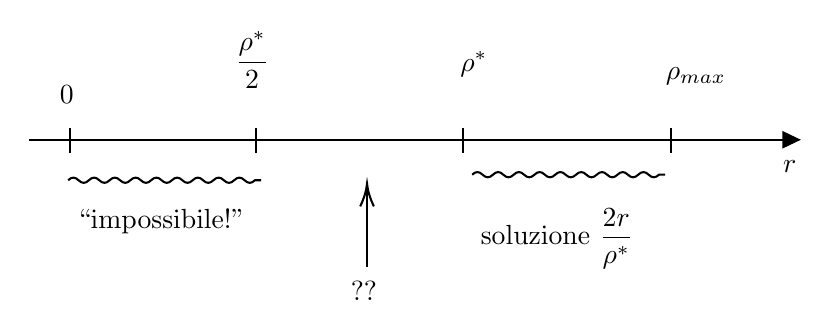
\begin{tikzpicture}[x=0.75pt,y=0.75pt,yscale=-1,xscale=1]
		%uncomment if require: \path (0,383); %set diagram left start at 0, and has height of 383

		%Straight Lines [id:da9485275221436212] 
		\draw    (121,120.5) -- (490,120.5) ;
		\draw [shift={(493,120.5)}, rotate = 180] [fill={rgb, 255:red, 0; green, 0; blue, 0 }  ][line width=0.08]  [draw opacity=0] (8.93,-4.29) -- (0,0) -- (8.93,4.29) -- cycle    ;
		%Straight Lines [id:da07537068280019232] 
		\draw    (230.33,115) -- (230.33,127) ;
		%Straight Lines [id:da2577463164839414] 
		\draw    (330.33,115) -- (330.33,127) ;
		%Straight Lines [id:da2779185025368248] 
		\draw    (430.33,115) -- (430.33,127) ;
		%Straight Lines [id:da7913738440257223] 
		\draw    (140.75,115) -- (140.75,127) ;
		%Straight Lines [id:da7607353200386405] 
		\draw    (140,140) .. controls (141.67,138.33) and (143.33,138.33) .. (145,140) .. controls (146.67,141.67) and (148.33,141.67) .. (150,140) .. controls (151.67,138.33) and (153.33,138.33) .. (155,140) .. controls (156.67,141.67) and (158.33,141.67) .. (160,140) .. controls (161.67,138.33) and (163.33,138.33) .. (165,140) .. controls (166.67,141.67) and (168.33,141.67) .. (170,140) .. controls (171.67,138.33) and (173.33,138.33) .. (175,140) .. controls (176.67,141.67) and (178.33,141.67) .. (180,140) .. controls (181.67,138.33) and (183.33,138.33) .. (185,140) .. controls (186.67,141.67) and (188.33,141.67) .. (190,140) .. controls (191.67,138.33) and (193.33,138.33) .. (195,140) .. controls (196.67,141.67) and (198.33,141.67) .. (200,140) .. controls (201.67,138.33) and (203.33,138.33) .. (205,140) .. controls (206.67,141.67) and (208.33,141.67) .. (210,140) .. controls (211.67,138.33) and (213.33,138.33) .. (215,140) .. controls (216.67,141.67) and (218.33,141.67) .. (220,140) .. controls (221.67,138.33) and (223.33,138.33) .. (225,140) .. controls (226.67,141.67) and (228.33,141.67) .. (230,140) -- (233,140) -- (233,140) ;
		%Straight Lines [id:da23941010014142017] 
		\draw    (334.67,137.33) .. controls (336.34,135.66) and (338,135.66) .. (339.67,137.33) .. controls (341.34,139) and (343,139) .. (344.67,137.33) .. controls (346.34,135.66) and (348,135.66) .. (349.67,137.33) .. controls (351.34,139) and (353,139) .. (354.67,137.33) .. controls (356.34,135.66) and (358,135.66) .. (359.67,137.33) .. controls (361.34,139) and (363,139) .. (364.67,137.33) .. controls (366.34,135.66) and (368,135.66) .. (369.67,137.33) .. controls (371.34,139) and (373,139) .. (374.67,137.33) .. controls (376.34,135.66) and (378,135.66) .. (379.67,137.33) .. controls (381.34,139) and (383,139) .. (384.67,137.33) .. controls (386.34,135.66) and (388,135.66) .. (389.67,137.33) .. controls (391.34,139) and (393,139) .. (394.67,137.33) .. controls (396.34,135.66) and (398,135.66) .. (399.67,137.33) .. controls (401.34,139) and (403,139) .. (404.67,137.33) .. controls (406.34,135.66) and (408,135.66) .. (409.67,137.33) .. controls (411.34,139) and (413,139) .. (414.67,137.33) .. controls (416.34,135.66) and (418,135.66) .. (419.67,137.33) .. controls (421.34,139) and (423,139) .. (424.67,137.33) -- (427.67,137.33) -- (427.67,137.33) ;
		%Straight Lines [id:da13829858178442833] 
		\draw    (284,181.67) -- (284,143.67) ;
		\draw [shift={(284,141.67)}, rotate = 450] [color={rgb, 255:red, 0; green, 0; blue, 0 }  ][line width=0.75]    (10.93,-3.29) .. controls (6.95,-1.4) and (3.31,-0.3) .. (0,0) .. controls (3.31,0.3) and (6.95,1.4) .. (10.93,3.29)   ;

		% Text Node
		\draw (483,129) node [anchor=north west][inner sep=0.75pt]   [align=left] {$\displaystyle r$};
		% Text Node
		\draw (134.5,93) node [anchor=north west][inner sep=0.75pt]   [align=left] {$\displaystyle 0$};
		% Text Node
		\draw (219,67) node [anchor=north west][inner sep=0.75pt]   [align=left] {$\displaystyle \frac{\rho ^{*}}{2}$};
		% Text Node
		\draw (327.5,76.5) node [anchor=north west][inner sep=0.75pt]   [align=left] {$\displaystyle \rho ^{*}$};
		% Text Node
		\draw (426.5,84) node [anchor=north west][inner sep=0.75pt]   [align=left] {$\displaystyle \rho _{max}$};
		% Text Node
		\draw (142.67,152.67) node [anchor=north west][inner sep=0.75pt]   [align=left] {``impossibile!''};
		% Text Node
		\draw (337.33,152) node [anchor=north west][inner sep=0.75pt]   [align=left] {soluzione $\displaystyle \frac{2r}{\rho ^{*}}$};
		% Text Node
		\draw (274.67,187.33) node [anchor=north west][inner sep=0.75pt]   [align=left] {??};


	\end{tikzpicture}
	\caption{Comportamento di \textsc{CenterSelectionPlus}.}
	\label{fig:csplus_r_beh}
\end{figure}
Quindi, ciò che succede dipende da $r$: se si sceglie maggiore o uguale a $\rho^*$
l'algoritmo produce una soluzione ammissibile con approssimazione $\frac{2r}{\rho^*}$.
Se $r \leq \frac{\rho^*}{2}$, l'algoritmo non produce soluzioni. Quando la scelta di
$r$ è $ \rho^*/2 < r < \rho^*$ l'algoritmo ha un comportamento sconosciuto,
ogni tanto produce soluzioni ammissibili e ogni tanto no. Noi non sappiamo il valore
di $r$, ma sappiamo che è sicuramente $r \in [0, \rho_{max}]$, dove $\rho_{max}$
è la distanza massima tra due punti. Una tecnica dicotomica (scegli un valore vicino a $0$,
se non produce nessun output alza la soglia minima e procedi con un valore vicino a $\rho_{max}$,
ripeti) può portare dei risultati.

\subsection{Algoritmo greedy center selection}
L'algoritmo \textit{greedy} per \textsc{CenterSelection} agisce come descritto
nell'algoritmo \ref{algo:GreedyCenterSelection}.
\begin{algorithm}[h]
	\caption{\textsc{GreedyCenterSelection}}
	\label{algo:GreedyCenterSelection}
	\KwInput{$S$, $k$, $d$}

	\If{$|S| \leq k$}
	{
		\Return $S$
	}

	$\hat{c} = extractRandomNode(S)$

	$C = \{\hat{c}\}$

	\While{$|C| \leq k$}
	{
		$\hat{c} = \arg \max_{S} d(s, C)$

		$C = C \cup \{\hat{c}\}$
	}
	\Return $C$
\end{algorithm}

\begin{theorem}
	L'algoritmo \textsc{GreedyCenterSelection} è $2$-approssimante.
\end{theorem}
\begin{proof}
	Per assurdo, supponiamo che $C$ sia $\rho(C) \geq 2\rho^*$, ossia
	esiste un $\hat{s} \in S$ tale che $d(\hat{s}, C) \geq 2\rho^*$.

	Consideriamo l'$i$-esima iterazione dell'algoritmo: sia $C_{\hat{i}}$ l'insieme
	dei centri all'inizio dell'$i$-esima iterazione e $c_{\hat{i}}$ il nuovo centro
	da inserire. Possiamo affermare che
	$$
		\forall s ~~ d(c_{\hat{i}}, C_{\hat{i}}) \geq d(s, C_{\hat{i}})
	$$
	e, in particolare, questo vale per $\hat{s}$:
	$$
		d(c_{\hat{i}}, C_{\hat{i}}) \geq d(\hat{s}, C_{\hat{i}}) \geq d(\hat{s}, C) > 2\rho^*
	$$
	il che implica che i $k$ cicli sono una delle esecuzioni possibili dei primi
	$k$ cicli dell'algoritmo, pertanto valgono tutte le proprietà che valevano
	per l'altro algoritmo per $r = \rho^*$. Siccome la distanza $d(\hat{s}, C) > 2\rho^*$
	il punto $\hat{s}$ non è ancora stato rimosso da $S$, quindi l'algoritmo deve
	ancora fare almeno un'iterazione, e allora l'algoritmo emetterà ``impossibile''.
	Questo è assurdo poiché per la proprietà $2$ di \textsc{CenterSelectionPlus}
	se $r \geq \rho^*$  allora l'algoritmo termina.
\end{proof}

\begin{theorem}
	Ammesso che $\mathbf{P} \neq \mathbf{NP}$, non esiste alcun algoritmo $\alpha$-approssimante
	per \textsc{CenterSelection} con $\alpha < 2$
\end{theorem}
\begin{proof}
	Per dimostrare questo teorema introduciamo brevemente il problema del \textsc{DominatingSet},
	un famoso problema di decisione NP-Completo.

	\prob {DominatingSet}
		{$G=(V, E)$ non orientato, $k \in \mathbb{N}$}
		{$\{0, 1\} = 2$}
		{Esiste $D \subseteq V$ con $|D| \leq k$ tale che sia un dominating set?}

	Diciamo che, dato un grafo $G=(V, E)$, un sottoinsieme $D \subseteq V$ è un \textsc{DominatingSet}
	di $G$ se e solo se $\forall x \in (V \setminus D)$ esiste un $y \in D$ vicino di $x$.

	\bigbreak

	Per assurdo, supponiamo che esista un algoritmo $\alpha$-approssimanete per \textsc{CenterSelection}
	con $\alpha < 2$.
	Sia $(G=(V, E), k)$ una istanza di \textsc{DominatingSet}, costruiamo una istanza di \textsc{CenterSelection}
	dove $S=V$, $k=k$ e la funzione distanza è definita in questo modo:
	$$
	d(x, y) =
	\begin{cases}
	 0 & \text{ se } x = y \\
	 1 & \text{ se } x \neq y \text{ e } (x, y) \in E \\
	 2 & \text{ altrimenti }
	\end{cases}
	$$

	È facile dimostrare che questa funzione rispetta le proprietà di uno spazio metrico: osservando la disuguaglianza
	triangolare abbiamo sul lato sinistro un valore che può essere 1 o 2, dal lato destro invece abbiamo la somma
	di due valori che possono essere entrambi anche loro o 1 o 2, dunque sempre maggiore o uguale al lato sinistro

	$$
		\underbrace{d(x, y)}_{\text{1 o 2}} <= \underbrace{\underbrace{d(x, z)}_{\text{1 o 2}} + \underbrace{d(z, y)}_{\text{1 o 2}}}_{\text{2 o 3 o 4}}
	$$

	In una istanza di \textsc{DominatingSet} convertita in \textsc{CenterSelection} dunque abbiamo che $\rho^*$ può
	assumere solo due valori: $1$ o $2$. Se $\rho^*=1$ è possibile dimostrare che $D$, l'insieme di centri scelti,
	è un dominating set nell'istanza originale del problema, tramite una semplice catena di implicazioni

	\begin{align*}
		\rho^*=1 &\leftrightarrow \forall x \in (V \setminus D) d(x, D) = 1 \\
				 &\leftrightarrow \forall x \in (V \setminus D), \exists y \in D \text{ tale che } d(x, y) = 1 \\
				 &\leftrightarrow \forall x \in (V \setminus D), \exists y \in D \text{ tale che } (x, y) \in E \\
				 &\leftrightarrow D \text{ è un \textsc{DominatingSet}}
	\end{align*}

	Eseguiamo il nostro algoritmo $\alpha$-approssimante per \textsc{CenterSelection}, con $\alpha < 2$ per ipotesi,
	sull'istanza convertita da \textsc{DominatingSet}. Abbiamo dunque che

	\begin{align*}
		1 \leq \frac{\rho}{\rho^*} \leq 2 - \varepsilon \\
		\rho^* \leq \rho \leq (2 - \varepsilon) * \rho^*
	\end{align*}

	Dato che $\rho^*$ può essere solamente $1$ o $2$, allora il nostro $\rho$ può ricadere in uno solo di due casi disgiunti:

	\begin{align*}
		1 \leq \rho \leq 2 - \varepsilon \implies \text{ esiste DominatingSet} \\
		2 \leq \rho \leq 4 - 2 \varepsilon \implies \text{ non esiste DominatingSet}
	\end{align*}

	Osservando quale delle due disequazioni il nostro $\rho$ soddisfa, potremmo decidere in tempo polinomiale
	se esiste o meno un \textsc{DominatingSet} per la nostra istanza. Questo sappiamo essere impossibile, dunque
	concludiamo che non possiamo approssimare di più \textsc{CenterSelection}.
\end{proof}


% lezione 5 - 13/10/2021
\section{Problema della copertura d'insiemi}
Prima di passare a descrivere il problema \textsc{SetCovering} è necessario
introdurre alcune proprietà delle funzioni armoniche.

\subsection{Funzioni armoniche}
Una funzione armonica è una funzione
$$
	H : \mathbb{N}^+ \rightarrow  \mathbb{R}
$$
ed è definita
$$
	H(n) = \sum_{k = 1}^{n} \frac{1}{k}
$$
per esempio $H(3) = 1 + 1/2 + 1/3$.
\begin{figure}[h]
	\centering
	\begin{subfigure}[b]{0.45\textwidth}
		\centering
		\begin{tikzpicture}
			\begin{axis}[
					xmin=0,
					xmax=4,
					ymin=0,
					ymax=3,
					samples=200,
					axis lines=left
				]

				\addplot [black] {1/x};

				\draw[pattern=north west lines] (0,0) rectangle (1,1);
				\draw[pattern=north west lines] (1,0) rectangle (2,1/2);
				\draw[pattern=north west lines] (2,0) rectangle (3,1/3);
				\draw[pattern=north west lines] (3,0) rectangle (4,1/4);
			\end{axis}
		\end{tikzpicture}
		\subcaption{Grafico di $f(x) = \frac{1}{x}$ verso aree delle somme in $H(4)$.}
	\end{subfigure}
	\hfill
	\begin{subfigure}[b]{0.45\textwidth}
		\centering
		\begin{tikzpicture}
			\begin{axis}[
					ymin=0,
					ymax=4,
					xmin=0,
					xmax=5,
					domain=0:4,
					samples=200,
					axis lines=left,
					clip=true,
					clip mode=individual]

				\addplot [black] {ln(x) + 1} node (plot1) {};
				\node [right] at (plot1) {$\ln(n) + 1$};

				\addplot [black] {ln(x + 1)} node (plot2) {};
				\node [right] at (plot2) {$\ln(n + 1)$};

				\draw[{Circle[open]}-,dashed] ({1,1}) -- ({1,1}|-{rel axis cs:0,0});
				\draw[{Circle[open]}-,dashed] ({2,3/2}) -- ({2,3/2}|-{rel axis cs:0,0});
				\draw[{Circle[open]}-,dashed] ({3,11/6,1}) -- ({3,11/6,1}|-{rel axis cs:0,0});
				\draw[{Circle[open]}-,dashed] ({4, 25/12,1}) -- ({4, 25/12,1}|-{rel axis cs:0,0});

			\end{axis}
		\end{tikzpicture}
		\subcaption{Grafico di $f(x) = \ln(x) + 1$ e $v(x) = \ln(x+1)$ verso i valori di $H(x)$ per i naturali $x = 1, 2, 3, 4$.}
	\end{subfigure}
	\caption{Proprietà di funzioni armoniche}
	\label{fig:1x_vs_harmo}
\end{figure}

\noindent
Le funzioni armoniche hanno delle proprietà:
\begin{lemma}\label{lem:harmo_leq_lnx}
	$$
		H(n) \leq 1 + \int_{1}^{n} \frac{1}{x} dx = 1 + \ln(x)|_1^n = 1 + \ln(n) - 0 = 1 + \ln(n)
	$$
\end{lemma}
\begin{lemma}\label{lem:harmo_geq_lnx1}
	In quanto
	$$
		\int_t^{t+1} \frac{1}{x} dx \leq \int_t^{t+1} \frac{1}{t} dx = \frac{1}{t}
	$$
	allora
	\begin{align*}
		 & H(n) = \frac{1}{1} + \frac{1}{2} + \cdots + \frac{1}{t} \geq \int_{1}^{2}\frac{1}{x} dx + \int_2^3 \frac{1}{x} dx + \cdots + \int_n^{n+1} \frac{1}{x} dx = \\
		 & = \int_1^{n+1}\frac{1}{x}dx = \ln(x)|_1^{n+1} = \ln(n+1)
	\end{align*}
	quindi $H(N) \geq \ln(n+1)$, e in conclusione
	$$
		\ln(n+1) \leq H(N) \leq 1 + \ln(n)
	$$
\end{lemma}

\noindent
Torniamo a descrivere il problema \textsc{SetCover}:

\popt {SetCover} {$S_1, S_2, \cdots, S_m \subseteq U$ tali che $\cup_{i = 1}^m S_i = U$
	e pesi $\forall i=1,\cdots, m ~~ w_i \in \mathbb{R}^{> 0}$ }
{Insieme di insiemi scelti (o indici) $C \subseteq \{1, \cdots, m\}$}
{Quali sono gli insiemi da scegliere per coprire tutti gli elementi di $U$ col
	costo minore possibile?} {$C$ tale che $\cup_{i \in C}S_i = U$}
{$Min$}{$w = \sum_{i \in C} w_i$}


\subsection{Algoritmo greedy set cover}
\begin{algorithm}[h]
	\caption{GreedySetCover}
	\label{algo:greedysetcover}
	\KwInput{$S_i, U$}

	$R = U$

	$S = \emptyset$

	\While{$R \neq \emptyset$}
	{
		$\hat{S} = \arg \min_{S_i} \{ \frac{w_i}{|S_i \cap R|}\}$

		$S = S \cup \{\hat{S}\}$

		$R = R \setminus \hat{S}$
	}
	\Return{$S$}

\end{algorithm}
Enunciamo e dimostriamo alcune proprietà dell'\cref{algo:greedysetcover};
inizialmente notiamo che ogni elemento $s \in U$ viene inserito in qualche
iterazione $j$ dell'algoritmo che sceglie un qualche $\hat{S}_j =S_{i_j}$. Definiamo
quindi
$$
	\forall u \in U ~~ c_u = \frac{w_{i_j}}{|S_{i_j} \cap R_j|}
$$
come il costo di ogni singolo elemento di $U$ coperto grazie alla scelta di $S_{i_j}$
durante la $j$-esima iterazione.

\begin{lemma}\label{lem:gsetcov_w_sum_c_u}
	$$
		w = \sum_{u \in U} c_u
	$$
\end{lemma}
\begin{proof}
	Supponiamo che la scelta $S = \{S_{i_1}, S_{i_2}, \cdots, S_{i_k}\}$ produca
	un costo
	$$
		w = w_{i_1} + w_{i_2} + \cdots + w_{i_k}
	$$
	con ogni $w_{i_j}$ il costo di ogni $S_{i_j}$ scelto alla $j$-esima iterazione.
	Gli elementi coperti alla $j$-esima iterazione sono esattamente i
	$u \in S_{i_j} \cap R_j$, che hanno
	$$
		c_u = \frac{w_{i_j}}{|S_{i_j} \cap R_j|}
	$$
	ed essendo in numero proprio $|S_{i_j} \cap R_j|$, si ottiene
	$$
		\sum_{u \in S_{i_j} \cap R_j} c_u = |S_{i_j} \cap R| \cdot \frac{w_{i_j}}{|S_{i_j} \cap R|} = w_{i_j}
	$$
	da cui si ottiene facilmente l'enunciato.
\end{proof}
\begin{lemma}\label{lem:gsetcov_cu_leq_harmoskwk}
	$$
		\forall k ~~ \sum_{u \in S_k} c_u \leq H(|S_k|) \cdot w_k
	$$
\end{lemma}
\begin{proof}
	Sia
	$$
		S_{i_j} = \{u_1, u_2, \cdots, u_d\}
	$$
	dove gli $u_i$ sono elencati in ordine di copertura, ossia all'inizio
	quelli che vengono coperti prima nell'algoritmo e alla fine quelli
	che verranno coperti dopo.
	Nell'iterazione $j$ in cui verrà coperto un certo $u_k \in S_j$ sarà
	$$
		\{u_k, \cdots, u_d\} \subseteq R_j
	$$
	e quindi deve necessariamente essere
	$$
		|S_{i_j} \cap R_j| \geq d - k + 1
	$$
	ossia rimangono almeno tanti elementi da coprire quanti quelli non ancora
	coperti di $S_{i_j}$ sin questo momento; pertanto
	\begin{align*}
		 & c_{u_k} = \frac{w_{j'}}{|S_{j'} \cap R_j|}   &  & \text{ con } j' \text{ potenzialmente diverso da } i_j \\
		 & \leq \frac{w_{i_j}}{|S_{i_j} \cap R_j|} \leq &  & \text{ poiché l'algoritmo sceglie il minimo}           \\
		 & \leq \frac{w_{i_j}}{d-k+1}
	\end{align*}

	Sommando per ogni $c_{u_i}$ si ha
	$$
		c_{u_1} + \cdots + c_{u_d} \leq \frac{w_{i_j}}{d-1 + 1} + \frac{w_{i_j}}{d-2+1} + \cdots + \frac{w_{i_j}}{d-d+1}
		= w_{i_j}(1 + \frac{1}{2} + \cdots + \frac{1}{d})
		= w_{i_j} \cdot H(|S_{i_j}|)
	$$
\end{proof}
\begin{theorem}
	Sia $M = \max{|S_i|}$. L'algoritmo \textsc{GreedySetCover} è una $H(M)$-approssimazione per
	il problema \textsc{SetCover}.
\end{theorem}
\begin{proof}
	Sia $w^* = \sum_{S_i \in S^*} w_i$.
	Allora, grazie al \cref{lem:gsetcov_cu_leq_harmoskwk}, abbiamo
	$$
		w_i \geq \frac{\sum_{u \in S_i} c_u}{H(|S_i|)} \geq \frac{\sum_{u \in S_i} c_u}{H(M)}
	$$
	Consideriamo il valore ottenuto sommando, per ogni insieme della copertura ottima $S^*$, la somma
	dei costi dei singoli elementi in ogni insieme. Questo valore è maggiore o uguale alla somma
	dei costi degli elementi nell'universo $U$, poichè nel primo valore potremmo sommare più volte
	il costo di alcuni elementi che compaiono in più insiemi scelti.
	Per il \cref{lem:gsetcov_w_sum_c_u} la seconda sommatoria è uguale al costo della soluzione ottima.
	$$
		\sum_{S_i \in S^*}\sum_{u \in S_i} c_u \geq \sum_{u \in U} c_u = w
	$$
	Applicando queste due osservazioni alla definizione di costo della soluzione ottima otteniamo
	\begin{align}
		 & w^* = \sum_{S_i \in S^*} w_i \geq \frac{\sum_{S_i \in S^*} \sum_{u \in S_i} c_u}{H(M)} \geq \frac{w}{H(M)} \\
		 & \implies \frac{w}{w^*} \leq H(M)
	\end{align}

	Inoltre, osservando che $M \leq |U| = n$, possiamo anche dire che:
	$$
		H(M) \leq H(n) = O(\ln(n))
	$$
\end{proof}
\begin{corollario}
	\textsc{GreedySetCover} è un algoritmo $O(\ln(n))-$approssimante.
\end{corollario}
Si può inoltre dimostrare che non esiste nessun algoritmo
$(1 - O(1))\ln(n)$-approssimante per il \textsc{SetCoverProblem},
ammesso che $\mathbf{P} \neq \mathbf{NP}$.

\begin{figure}[h]
	\centering

	\tikzset{every picture/.style={line width=0.75pt}} %set default line width to 0.75pt        

	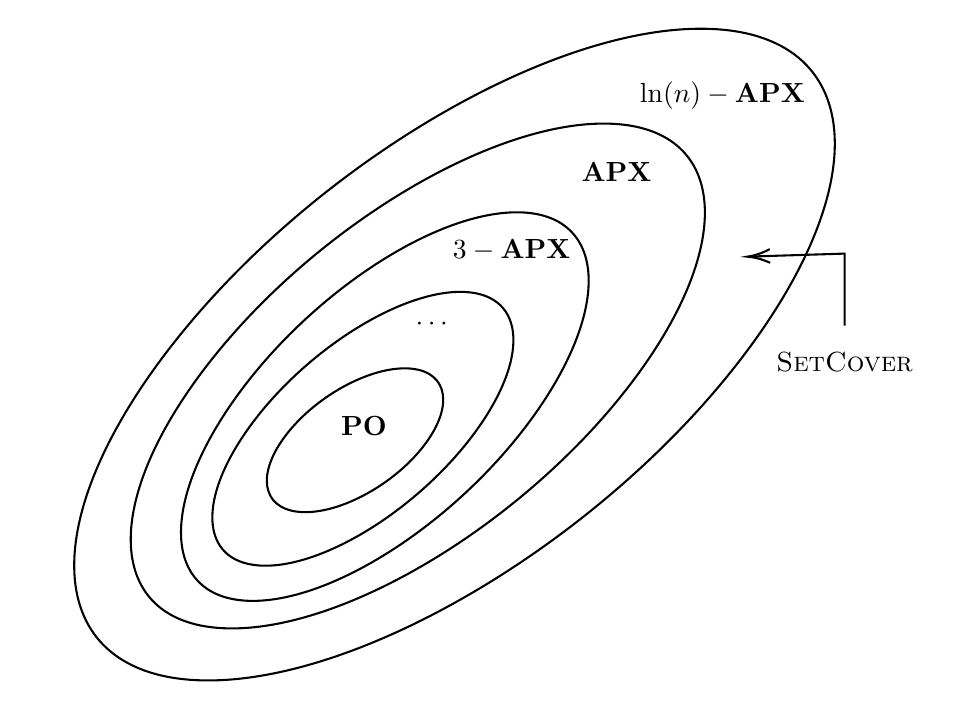
\begin{tikzpicture}[x=0.75pt,y=0.75pt,yscale=-1,xscale=1]
		%uncomment if require: \path (0,477); %set diagram left start at 0, and has height of 477

		%Shape: Ellipse [id:dp4588658322810296] 
		\draw   (310.61,174.5) .. controls (376.13,87.79) and (491.77,17.5) .. (568.88,17.5) .. controls (645.98,17.5) and (655.37,87.79) .. (589.84,174.5) .. controls (524.31,261.21) and (408.68,331.5) .. (331.57,331.5) .. controls (254.46,331.5) and (245.08,261.21) .. (310.61,174.5) -- cycle ;
		%Shape: Ellipse [id:dp4441062862246874] 
		\draw   (327.15,184.82) .. controls (376.62,117.65) and (463.91,63.2) .. (522.11,63.2) .. controls (580.32,63.2) and (587.41,117.65) .. (537.94,184.82) .. controls (488.48,251.99) and (401.19,306.44) .. (342.98,306.44) .. controls (284.77,306.44) and (277.68,251.99) .. (327.15,184.82) -- cycle ;
		%Shape: Ellipse [id:dp42532014972954124] 
		\draw   (341.82,199.56) .. controls (376.94,147.86) and (438.92,105.95) .. (480.25,105.95) .. controls (521.58,105.95) and (526.61,147.86) .. (491.49,199.56) .. controls (456.37,251.26) and (394.39,293.17) .. (353.06,293.17) .. controls (311.73,293.17) and (306.7,251.26) .. (341.82,199.56) -- cycle ;
		%Shape: Ellipse [id:dp9403889034822421] 
		\draw   (350.81,210.25) .. controls (376.75,173.81) and (422.52,144.28) .. (453.04,144.28) .. controls (483.57,144.28) and (487.28,173.81) .. (461.34,210.25) .. controls (435.4,246.68) and (389.63,276.22) .. (359.11,276.22) .. controls (328.58,276.22) and (324.87,246.68) .. (350.81,210.25) -- cycle ;
		%Shape: Ellipse [id:dp9056149450292196] 
		\draw   (367.2,215.78) .. controls (380.43,196.64) and (406.86,181.13) .. (426.24,181.13) .. controls (445.62,181.13) and (450.6,196.64) .. (437.38,215.78) .. controls (424.15,234.91) and (397.71,250.42) .. (378.34,250.42) .. controls (358.96,250.42) and (353.97,234.91) .. (367.2,215.78) -- cycle ;
		%Straight Lines [id:da10034962558485494] 
		\draw    (638.18,160.5) -- (638.18,125.85) -- (593.29,127.26) ;
		\draw [shift={(591.29,127.33)}, rotate = 358.2] [color={rgb, 255:red, 0; green, 0; blue, 0 }  ][line width=0.75]    (10.93,-3.29) .. controls (6.95,-1.4) and (3.31,-0.3) .. (0,0) .. controls (3.31,0.3) and (6.95,1.4) .. (10.93,3.29)   ;

		% Text Node
		\draw (538.07,41.64) node [anchor=north west][inner sep=0.75pt]   [align=left] {$\ln(n)-\mathbf{APX}$};
		% Text Node
		\draw (510,80.38) node [anchor=north west][inner sep=0.75pt]   [align=left] {$\mathbf{APX}$};
		% Text Node
		\draw (448,117.56) node [anchor=north west][inner sep=0.75pt]   [align=left] {$3-\mathbf{APX}$};
		% Text Node
		\draw (430,155.6) node [anchor=north west][inner sep=0.75pt]   [align=left] {$\cdots$};
		% Text Node
		\draw (394.14,202.63) node [anchor=north west][inner sep=0.75pt]   [align=left] {$\mathbf{PO}$};
		% Text Nodej
		\draw (638.18,178) node   [align=left] {\begin{minipage}[lt]{51.43pt}\setlength\topsep{0pt}
				\begin{center}
					\textsc{SetCover}
				\end{center}

			\end{minipage}};

	\end{tikzpicture}
	\caption{\textsc{SetCover} $\in \ln(n)-\mathbf{APX}$.}
	\label{fig:setcoverapx}
\end{figure}



% lezione 6 - 15/10/2021
\begin{theorem}
	Il lower bound $O(\log(n))$ è \textit{stretto}.
\end{theorem}
\begin{proof}
	Il teorema si dimostra creando un input ``cattivo'':
	% TODO!
	%disegno insiemi...
\end{proof}
La particolarità tecnica interessante risiede nell'analisi di complessità:
abbiamo attribuito ad ogni singolo elemento un costo; questa tecnica, che
si chiama \textit{pricing}, è a volte utile anche per il design degli algoritmi.

\section{Problema della copertura dei vertici}
\popt {VertexCover} {$G = (V,E)$ non diretto, con pesi
	$\forall i \in V ~ w_i \in \mathbb{Q}^{>0}$}
{Insieme di vertici $X \subseteq V$}
{Quale è il numero minimo di vertici da selezionare per coprire ogni lato?}
{$X \subseteq V$ tale che $\forall e \in E ~ e \cap X \neq \emptyset$}
{$Min$}{$w = \sum_{i \in X} w_i$}

\subsection{Relazione tra vertex e set cover}
\begin{theorem}\label{thm:vc_polyred_sc}
	Ogni istanza del problema di decisione associato $\hat{\Pi}_{VC}$ del problema \textsc{VertexCover} è
	polinomialmente riducibile ad una istanza del problema di decisione associato
	$\hat{\Pi}_{SC}$ di \textsc{SetCover}, ossia
	$$
		\hat{\Pi}_{VC} \leq_p \hat{\Pi}_{SC}
	$$
\end{theorem}
\begin{proof}
	Supponiamo di avere un'istanza $(G=(V,E), w_i, w_{max})$ di
	$\hat{\Pi}_{VC}$; si può trasformare nell'istanza
	$(S= \{S_1, S_2, \cdots, S_n\}, w_i, w_{max})$ di $\hat{\Pi}_{SC}$ 
	definendo l'universo $U=E$ e creando un $S_i$ per ogni vertice $i \in V$ tale che 
	$S_i = \{e \in E | e \text{ incide su } i\}$.
\end{proof}

Di fatto, se abbiamo un algoritmo per
risolvere \textsc{SetCover} con un fattore di approssimazione, allora possiamo
risolvere anche \textsc{VertexCover} con lo stesso fattore;
questo, ovviamente, non è necessariamente il caso generale: dati due problemi
$\hat{\Pi}_1 \leq_p \hat{\Pi_2}$ e un algoritmo che risolve con un certo fattore
di approssimazione $\hat{\Pi_2}$, non è detto che esso risolva
\textit{con lo stesso fattore di approssimazione} un'istanza di $\hat{\Pi_1}$.

\begin{theorem}
	\textsc{VertexCover} è $H(D)$-approssimabile (dove $D$ è il grado massimo)
	utilizzando la riduzione polinomiale verso \textsc{SetCover}.
\end{theorem}

\subsection{Algoritmo basato su pricing}
Sia l'istanza di \textsc{VertexCover} formata da $G = (V,E)$ un grafo e
$\langle w_i \rangle_{i \in V}$ un'insieme di costi definiti
sui vertici; diciamo che un \textit{assegnamento di prezzi} sui lati
$\langle P_e \rangle_{e \in E}$ è \textbf{equo} se e solo se
$$
	\forall i \in V \sum_{e \text{ incidente su } i} P_e \leq w_i
$$
e l'assegnamento si definisce \textit{stretto} su un vertice $i$ se
$$
	\sum_{e \text{ incidente su } i} P_e = w_i
$$
\begin{lemma}\label{lem:vcov_pricing_eq_sum_p_e_w_opt}
	Se $\langle P_e \rangle_{e \in E}$ è un sistema di prezzi equo, allora
	$$
		\sum_{e \in E} P_e \leq w^*
	$$
	dove $w^*$ il costo ottimo per l'istanza di \textsc{VertexCover}.
\end{lemma}

\begin{proof}
	Per l'equità sappiamo che
	$$
		\forall i \in V ~ \sum_{e \text{ incidente su } i} P_e \leq w_i
	$$
	Sia quindi $X^*\subseteq V$ una soluzione ottima, sommiamo tutti i prezzi 
	degli archi incidenti sui vertici di $X^*$:
	$$
		\sum_{i \in X^*} \sum_{e \text{ incidente su } i} P_e \leq \sum_{i \in X^*} w_i = w^*
	$$
	Dato che $X^*$ è una soluzione, tutti i lati del grafo incidono su almeno
	uno dei suoi vertici, possiamo dunque dire
	$$
		\sum_{e \in E} P_e \leq \sum_{i \in X^*} \sum_{e \text{ incidente su } i} P_e
	$$
	Osservando i lati della disuguaglianza completa otteniamo il lemma:
	$$
		\sum_{e \in E} P_e \leq \sum_{i \in X^*} \sum_{e \text{ incidente su } i} P_e \leq \sum_{i \in X^*} w_i = w^* \\
	$$
\end{proof}
\begin{algorithm}
	\caption{\textsc{PricedVertexCover}}
	\label{algo:PricedVertexCover}
	\KwInput{$G(V,E)$, $w_i$}

	\For{$e \in E$}
	{
		$P_e = 0$
	}

	\While{$\exists \bar{e} = \{\bar{i},\bar{j}\}$ t.c. $P_{\bar{e}}$ non è stretto né su $\bar{i}$ né su $\bar{j}$}
	{
		$\Delta = \min\{w_{\bar{i}} - \sum_{e \text{ incidente su } \bar{i}} P_e, w_{\bar{j}} - \sum_{e \text{ incidente su } \bar{j}} P_e\}$

		$P_{\bar{e}} = P_{\bar{e}} + \Delta$
	}

	$S = \{v \in V | \langle P_e \rangle \text{ è stretto su } v\}$

	\Return {$S$}
\end{algorithm}

\begin{lemma}\label{lem:pvcov_w_le_w_sum_P_e}
	Al termine dell'esecuzione, per l'\cref{algo:PricedVertexCover} vale
	$$
		w \leq 2 \sum_{e \in E} P_e
	$$
\end{lemma}
\begin{proof}
	Abbiamo che
	$$
		w = \sum_{i \in S} w_i \text { e } 
	$$
	inoltre, dato che l'insieme $S$ dato in output dall'algoritmo contiene per definizione
	solo vertici stretti, vale anche
	$$
		\forall i \in S ~ w_i = \sum_{e \text{ inc. su } i} P_e
	$$
	quindi
	$$
		w = \sum_{i \in S} \sum_{e \text{ inc. su } i} P_e
	$$
	Per come è fatta la somma, ogni $e$ appare 1 o 2 volte in base a se solo uno o entrambi
	dei suoi vertici sono stretti. Approssimando per eccesso dunque possiamo dire che
	$$
		w \leq 2 \sum_{e \in E} P_e
	$$
\end{proof}

\begin{theorem}
	\textsc{PricedSetCover} è un algoritmo $2$-approssimante per \textsc{VertexCover}.
\end{theorem}

\begin{proof}
	$$
		\frac{w}{w^*} \underbrace{\leq}_\text{\cref{lem:pvcov_w_le_w_sum_P_e}}
		\frac{2\sum_{e \in E} P_e}{w^*}
		\underbrace{\leq}_\text{\cref{lem:vcov_pricing_eq_sum_p_e_w_opt}}
		\frac{2 \sum_{e \in E} P_e}{\sum_{e \in E} P_e} = 2
	$$
\end{proof}

% ---- MOVED  ---------------------------------------------------------------
% lezione 7 - 20/10/2021
% refresher sulla dimostrazione precedente
% dimostrazione della correttezza dell'algoritmo...
% definiamo un grafo "doppio ventaglio": s->a0, s->a1, ..., s->a_{k-1} 
% each a_{i}->x x->y y->b0, y->b1, ..., y->b_{k-1}, 
% each b_{i}->t. Se (s,t) compare due volte, il bridge (x, y) è selezionato 
% la prima volta e non dovrebbe essere in grado di completare il compito.
% --------------------------------------------------------------------------

\subsection{Algoritmo basato sull'arrotondamento}
Per poter utilizzare questa tecnica, è necessario introdurre alcune nozioni
aggiuntive.
\subsubsection{Programmazione lineare}
\popt {LinearProgramming}
{Una matrice $A \in \mathbb{Q}^{m \times n}$ che rappresenta gli $m$ vincoli
	per $n$ variabili, un vettore $\mathbf{b} \in \mathbb{Q}^{m}$ che rappresenta i
	termini noti e un terzo vettore $\mathbf{c} \in \mathbb{Q}^m$ usato per la
	funzione obiettivo}
{Un vettore $\mathbf{x} \in \mathbb{Q}^n$}
{Qual è il vettore $\mathbf{x}$ che implica il costo minore?}
{$\mathbf{x}\in \mathbb{Q}^{n}$ tale che $A \mathbf{x} \geq \mathbf{b}$}
{$Min$}
{ $\mathbf{c}^T \mathbf{x}$ }

\subsubsection{Programmazione lineare intera}
\popt {IntegerLinearProgramming}
{Una matrice $A \in \mathbb{Q}^{m \times n}$, un vettore $\mathbf{b} \in \mathbb{Q}^{m}$
	e un vettore $\mathbf{c} \in \mathbb{Q}^b$}
{Un vettore $\mathbf{x} \in \mathbb{Z}^n$}
{Qual è il vettore $\mathbf{x}$ che implica il costo minore?}
{$\mathbf{x}\in \mathbb{Z}^{n}$ tale che $A \mathbf{x} \geq \mathbf{b}$}
{$Min$}
{ $\mathbf{c}^T \mathbf{x}$ }

\`E chiaro che, per lo stesso input, una soluzione per \textsc{IntegerLinearProgramming}
è peggiore o uguale ad ogni soluzione per \textsc{LinearProgramming}, in quanto una
soluzione per quest'ultimo potrebbe utilizzare anche lo spazio di valori frazionari
per ottenere una soluzione migliore. La trasformazione di un problema da \textsc{IntegerLinearProgramming}
in un problema in \textsc{LinearProgramming} è detto \textit{rilassamento}.

Per lungo tempo non si è saputo se \textsc{LinearProgramming} fosse risolvibile in tempo polinomiale:
oggi, si sa che è risolvibile in tempo polinomiale nella dimensione dell'input e nel numero di vincoli.
\begin{theorem}\label{thm:LinearProgramming_PO}
	\textsc{LinearProgramming} $\in \mathbf{PO}$.
\end{theorem}

Uno degli esempi dei metodi polinomiali è il \textit{metodo del punto interno}
di Karmarkar. Questi metodi sono molto complicati da implementare e benché siano
dimostrabilmente polinomiali, spesso sono meno efficienti di algoritmi che
non sono dimostrabilmente polinomiali come l'\textbf{algoritmo di Dantzig}.

Per quanto riguarda ILP, invece, la situazione è diversa.
\begin{theorem}\label{thm:IntegerLinearProgramming_NPOc}
	\textsc{IntegerLinearProgramming} $\in \mathbf{NPO-completi}$.
\end{theorem}

\begin{proof}
	Per assurdo, assumiamo che esista un algoritmo che risolva 
	\textsc{IntegerLinearProgramming} in tempo polinomiale, e di conseguenza
	anche il suo problema di decisione associato.
	Possiamo dare una riduzione in tempo polinomiale di una istanza del problema
	di decisione \textsc{VertexCover} in una istanza del problema di decisione
	\textsc{IntegerLinearProgramming}.

	Dati $n$ nodi con costi $v_0, \cdots, v_n$ e $m$ archi, vogliamo scegliere
	il numero massimo di nodi tale che il costo sia minimo e tutti gli archi
	siano coperti. Per tradurre questo in un problema di programmazione lineare
	intera, generiamo una variabile binaria per ogni nodo:
	$$
		x_i = \begin{cases} 0 & \text{ il vertice } i \text{ non è stato scelto} \\
              	1 & \text{ il vertice } i \text{ è stato scelto}\end{cases}
	$$
	Imponiamo i seguenti vincoli sulle variabili $x_i$:
	$$
		\begin{cases}
			x_i + x_j \geq 1 & \forall i, j \in E \\
			x_i \geq 0       & \forall i \in V    \\
			x_i \leq 1       & \forall i \in V
		\end{cases}
	$$
	La funzione obiettivo per il problema \textsc{IntegerLinearProgramming}$(G,w)$
	così costruito sarà
	$$
		\sum_{i \in V} w_i x_i
	$$

	Se riuscissimo a risolvere tutti i problemi di $\hat{\textsc{IntegerLinearProgramming}}$
	in tempo polinomiale allora potremmo risolvere anche $\hat{\textsc{VertexCover}}$ in tempo
	polinomiale. Dato che $\hat{\textsc{VertexCover}} \in \mathbf{NP-Completi}$ concludiamo
	che anche $\hat{\textsc{IntegerLinearProgramming}} \in \mathbf{NP-Completi}$ e dunque
	anche $\textsc{IntegerLinearProgramming} \in \mathbf{NPO-Completi}$.
\end{proof}

Essendo nell'insieme $\mathbf{NPO}-completi$, ogni problema è polinomialmente riducibile
ad un'istanza di \textsc{IntegerLinearProgramming}; ciò che a volte accade è
che anche la versione rilassata, ossia un'istanza di \textsc{LinearProgramming},
abbia una relazione col problema originale: questo è ciò che faremo con
\textsc{VertexCover}.

Data un'istanza $\Pi_{VC}$, una soluzione per la sua riduzione $\Pi_{ILP}$ è
una soluzione \textbf{esatta} anche per l'istanza originale (per la $\mathbf{NP}-$completezza
di quest'ultimo problema).
Se, ora, si rilassa il vincolo di interezza, ossia
$$
	\forall x, x_i \in \mathbb{Q}
$$
mantenendo le condizioni
$$
	\begin{cases}
		x_i + x_j \geq 1 & \forall i, j \in E \\
		x_i \geq 0                            \\
		x_i \leq 1
	\end{cases}
$$
si ottiene  un'istanza \textit{rilassata}, ossia \textsc{LinearProgramming}$(G,w)$,
che è risolvibile polinomialmente (ma non è detto che la soluzione sia
esatta anche per il problema originale).

Abbiamo, da quanto detto precedentemente
\begin{lemma}\label{lem:lp_leq_ilp}
	$$
		w^*_{LP} \leq w^*_{ILP}
	$$
\end{lemma}

Per sfruttare la programmazione lineare per risolvere un'istanza di
\textsc{VertexCover}, è necessario innanzitutto trasformarla in un problema
di programmazione lineare (non intera); a questo punto è possibile
risolvere l'istanza in tempo polinomiale ottenendo una soluzione $\mathbf{x}^*$;
definiamo la soluzione per l'istanza iniziale $\mathbf{r}$ come segue:
$$
	\forall i \in V ~~  r_i =
	\begin{cases}
		1 & x_i \geq \frac{1}{2} \\
		0 & x_i < \frac{1}{2}
	\end{cases}
$$
\begin{lemma}\label{lem:ilp_r_ammiss}
	La soluzione $\mathbf{r}$ è ammissibile per \textsc{IntegerLinearProgramming}.
\end{lemma}
\begin{proof}
	Deve essere $\forall i, j \in E ~ r_i+r_j \geq 1$.
	Per assurdo, assumiamo che $\exists i, j \in E$ tali che $r_i + r_j < 1$.
	Allora deve necessariamente essere che $r_i = r_j = 0$, poiché altrimenti
	la somma sarebbe già uguale a $1$. Quindi
	\begin{align*}
		 & x_i^* \leq \frac{1}{2} \land x_j^* \leq \frac{1}{2} \\
		 & \implies x_i^* +x_j^* < 1
	\end{align*}
	Ma questo è impossible, perché nel problema di programmazione lineare
	c'è il vincolo che per ogni arco la somma delle due variabili
	corrispondenti fosse maggiore o uguale a $1$ -- in altre parole,
	$x^*$ stessa non sarebbe una soluzione ammissibile per \textsc{LinearProgramming}.
\end{proof}
\begin{lemma} \label{lem:ilp_r_i_leq_2_x_i}
	$$ \forall i \in V ~~ r_i \leq 2x_i^*$$
\end{lemma}
\begin{proof}
	Se $r_i = 0$ la disuguaglianza è ovvia;
	se $r_i  = 1$ allora, $x^*_i \geq \frac{1}{2}$  e $2x_i^* \geq 1 = r_i$.
\end{proof}
\begin{lemma}\label{lem:ilp_appr}
	$$
		\sum_{i \in V} w_i r_i \leq 2 \sum_{i \in V} w_i x_i^* = 2w^*_{LP} \leq 2w^*_{ILP}
	$$
\end{lemma}
\begin{proof}
	Diretta dal \cref{lem:lp_leq_ilp}.
\end{proof}
\begin{theorem}
	L'utilizzo di \textsc{LinearProgramming} per risolvere problemi di \textsc{VertexCover}
	porta ad un algoritmo $2$-approssimante.
\end{theorem}
\begin{proof}
	Diretta dal \cref{lem:ilp_appr}.
\end{proof}
% ----------------- END MOVED -----------------------------------------------

\section{Problema dei cammini disgiunti}
\popt {DisjointPaths} {$G = (N,A)$ orientato, $k$ coppie
	$(s_1, t_1), \cdots, (s_k,t_k) \in \mathbb{N} \times \mathbb{N}$ e
	$c \in \mathbb{N}$}
{Un insieme di cammini}
{Quante coppie possono essere collegate senza utilizzare nessun lato più di $c$ volte?}
{$I \subseteq \{1,\cdots,k\}$ e, per ogni $i \in I$, un cammino $\Pi_i : s_i \leadsto t_i$
	tale che nessun $a \in A$ sia usato da più di $c$ cammini}
{$Max$}{Cardinalità dell'insieme $I$, $|I|$}

Dato un grafo orientato $G=(N,A)$, il problema consiste nel collegare più
coppie possibili senza usare nessun lato più di $c$ volte.
Anche in questo caso potremo usare un'algoritmo basato sulla tecnica
del pricing: ogni lato avrà, nell'esecuzione di questo algoritmo,
un prezzo che aumenterà durante l'esecuzione (più un lato è congestionato,
più vogliamo che venga scelto raramente).
Il problema è di massimo, ossia vogliamo collegare più coppie possibili.

\subsection{Algoritmo basato su pricing}
Oltre al grafo $G$, le $k$ coppie e il numero $c$ di utilizzi massimi per ogni lato,
l'algoritmo utilizza un parametro $\beta$ e una funzione di costo
$$
	l: A \rightarrow \mathbb{R}^{>0}
$$
estensibile ai cammini, ossia dato un cammino
$$
	\pi = \langle x_1, x_2, \cdots, x_k \rangle
$$
si definisce
$$
	l(\pi) = l(x_1, x_2) + l(x_2, x_3) + \cdots
$$
Il listato è esposto nell'\cref{algo:PricedDisjointPaths}.
Per dimostrare che esso è polinomiale, ricordiamo che Dijkstra richiede
tempo $O(m \log(n))$; ripetuto $k$ volte il costo di \textsc{PricedDisjointPaths}
è $O(k m \log (n))$.

\begin{algorithm}
	\caption{PricedDisjointPaths}
	\label{algo:PricedDisjointPaths}
	\KwInput{coppie $(s_i, t_i)$, $\beta$, $G=(N,A)$, $l$}

	$I = \emptyset$ \tcc*{insieme di coppie}

	$P = \emptyset$ \tcc*{insieme di cammini}

	\For{$a \in A$}
	{
		$l(a) = 1$
	}
	\While{$true$}
	{

		\tcc{trova il più corto cammino $\pi_i$ rispetto a $l$ che
			connette delle coppie $(s_i, t_i)$ tali che $i \notin I$}

		$ \pi_i = MinPath(l, (s_i, t_i) )$
		\If {$!\pi_i$}
		{

			\Return {I, P}

		}

		$I = I \cup \{i\}$

		$P = P \cup \{\pi\}$

		\tcc{aggiorna i costi che pesano su ogni arco: se superano
			il massimo, rimuovili in modo che non vengano più scelti}

		\For{$a \in \pi_i$}
		{

			$l(a) = l(a) \cdot \beta $


			\If {$l(a) = \beta^c$}
			{
				$\mathbf{delete} ~ a$
			}
		}
	}

\end{algorithm}

\noindent
Con lo scopo di esplorare alcuni aspetti dell'algoritmo, diamo alcune
definizioni: fissata la funzione $l(\cdot)$, definiamo un cammino $\pi$
\textbf{corto} se e solo se $l(\pi) \leq \beta^c$; inoltre, un cammino $\pi$ è
definito \textbf{utile} \textit{in un determinato momento dell'esecuzione dell'algoritmo}
se e solo se collega una coppia $i \notin I$.

\begin{lemma}\label{lem:priceddpaths_su}
	Durante l'algoritmo, finché esistono cammini utili e corti,
	l'algoritmo sceglie uno di essi.
\end{lemma}
\begin{proof}
	Siccome l'algoritmo sceglie tra tutti i cammini utili quello più corto,
	è chiaro che se c'è un cammino di costo minore di $\beta^c$ l'algoritmo
	non andrà mai a sceglierne uno lungo.
\end{proof}

Inoltre, come osservazione marginale, durante la prima fase dell'esecuzione
dell'algoritmo possiamo evitare di cancellare gli archi: si supponga di non
cancellare gli archi finché l'algoritmo ha modo di scegliere i cammini corti;
si supponga quindi che per errore venga scelto un cammino \textit{corto}
che passa per un arco già utilizzato $c$ volte. Questo è impossibile, poiché
se quel cammino contiene un arco già utilizzato $c$ volte, il suo costo è
maggiore o uguale a $\beta^c$, pertanto non è corto.

Quando la disponibilità di cammini corti termina, l'algoritmo si ferma
oppure comincia a scegliere dei cammini lunghi. A noi interessa proprio lo
stato del sistema in questo momento: sia quindi $c_t$ l'insieme dei cammini
\textit{utili} e \textit{corti} all'inizio della $t$-esima
iterazione. \`E chiaro che sia
$$
	c_0 \supseteq c_1 \supseteq \cdots \supset c_{t}
$$
poiché un cammino utile e corto può diventare (o essere rimpiazzato da
un altro, a causa dell'eliminazione degli archi) inutile o lungo.
Può accadere quindi che ad una certa iterazione $\bar{t}$ che sia $c_{\bar{t}} = \emptyset$;
chiamiamo quindi $\bar{l}$ la funzione $l$ a tale iterazione (o, se non accade,
al termine dell'esecuzione). Sia quindi $\bar{P} \subseteq P$ l'insieme dei cammini $\bar{l}$-corti
nell'output e $\bar{I} \subseteq I$ l'insieme delle coppie collegate da tali cammini.

\begin{lemma}\label{lem:priceddpaths_non_included_non_short}
	Sia $i \in I^* \setminus I$. Si ha $\bar{l}(\pi_{i}^*) \geq \beta^c$; in altre
	parole il costo di un cammino ottimo per una coppia che non è stato incluso
	nella soluzione dall'algoritmo è, all'istante $\bar{t}$, maggiore o uguale
	di $\beta^c$.
\end{lemma}
\begin{proof}
	Se così non fosse, allora $\pi_*$ sarebbe corto e, in quel momento, utile,
	pertanto verrebbe selezionato, contraddicendo l'ipotesi iniziale.
	In altre parole, $\pi_{i}^*$ resta utile fino alla fine;
	se fosse $\bar{l}(\pi_i^*) < \beta^c$, allora $\pi_i^*$ sarebbe corto nell'istante $\bar{t}$.
\end{proof}

\begin{lemma}\label{lem:priceddpaths_sum_l_a_leq_bc_i_m}
	$$
		\sum_{a \in A} \bar{l}(a) \leq \beta^{c+1} |\bar{I}| + m
	$$
\end{lemma}
\begin{proof}
	\begin{itemize}
		\item per $t = 0$, $\sum_{a \in A} l_0(a) = \sum_{a \in A} 1  = m$
		\item consideriamo il $j$-esimo passo, in cui si modificano i pesi
		      di alcuni archi modificando la funzione $l_{j}$ creando
		      $l_{j+1}$ in questo modo:
		      $$
			      l_{j+1}(a) =
			      \begin{cases}
				      l_j(a)             & \text{se } a \notin \pi_i \\
				      \beta \cdot l_j(a) & \text{se } a \in \pi_i
			      \end{cases}
		      $$
		      Possiamo quindi calcolare la differenza di prezzi degli archi
		      nel passaggio tra iterazioni:
		      \begin{align*}
			       & \sum_{a\in A} l_{j+1}(a) - \sum_{a \in A} l_j (a) = \sum_{a \in A} (l_{j+1}(a) - l_{j}(a)) =      \\
			       & \underbrace{\sum_{a \in A\setminus{\pi}} 0}_{\text{nessun cambio di peso negli archi non in }\pi}
			      + \sum_{a \in \pi}(\beta l_{j}(a) - l_{j}(a)) =                                                      \\
			       & = \sum_{a \in \pi_i} (\beta -1 ) l_j (a) \leq \beta \sum_{a \in \pi_i}l_j(a)
		      \end{align*}
			  Sappiamo dal \cref{lem:priceddpaths_non_included_non_short} che 
			  tutti i $\pi$ aggiunti fino al passo corrispondente a $\bar{l}$
			  sono cammini utili e corti, dunque abbiamo che
			  $$
			  	  \beta \underbrace{\sum_{a \in \pi_i}l_j(a)}_{\leq \beta^c \text{ dato che è un cammino utile}} \leq \beta^{c + 1}
			  $$
	\end{itemize}
	Abbiamo dunque che alla prima iterazione il peso totale degli archi è $m$
	mentre in quelle successive abbiamo un incremento nel peso totale degli archi 
	di un valore $\leq \beta^{c+1}$. Sappiamo che ad ogni iterazione 
	corrisponde l'aggiunta di un singolo cammino $\pi \in \bar{I}$, dunque $|\bar{I}|$ è
	anche il numero di iterazioni fatte dall'algoritmo quando la funzione di costo è $\bar{l}$. 
	Mettendo insieme queste osservazioni concludiamo che
	$$
	    \sum_{a \in A} \bar{l}(a) \leq \beta^{c+1} |\bar{I}| + m
	$$
\end{proof}

\begin{corollario}\label{cor:priceddpaths_cor_1}
	Dal \cref{lem:priceddpaths_non_included_non_short} abbiamo
	$$
		\sum_{i \in I^* \setminus I} \bar{l}(\pi_i^*) \geq \beta^c |I^*\setminus I|
	$$
\end{corollario}

\begin{corollario}\label{cor:priceddpaths_cor_2}
	\begin{align*}
		 & \sum_{i \in I^* \setminus I} \bar{l}(\pi_i^*) \leq \sum_{i \in I^*}\bar{l}(\pi_i^*) \leq c \sum_{a \in A} \bar{l}(a) &  & \text{ poiché  } I^* \text{ è una soluzione ogni arco è usato al più } c \text { volte}           \\
		 & \leq c (\beta^{c+1}|\bar{I}|+m)                                                                                      &  & \text{ dal \cref{lem:priceddpaths_sum_l_a_leq_bc_i_m}}
	\end{align*}
\end{corollario}

\begin{theorem}\label{thm:priceddpaths_approx}
	\textsc{PricedDisjointPaths} è un algoritmo $O(1 + 2cm^{\frac{1}{c+1}})-$approssimante per
	\textsc{DisjointPaths}.
\end{theorem}
\begin{proof}
	Dalle proprietà degli insiemi è possible affermare che
	\begin{align*}
		 & \beta^c |I^*| = \beta^c |I^* \cap I| + \beta^c |I^* \setminus I| \leq                                                                                         \\
		 & \leq \beta^c|I^*\cap I| + \sum_{i \in I^* \setminus I} \bar{l}(\pi_i^*)                                        &  &
		\text{ dal \cref{cor:priceddpaths_cor_1}}                                                                                                                        \\
		 & \leq \beta^c |I| + \sum_{i \in I^* \setminus I} \bar{l}(\pi_i^*) \leq \beta^c |I| + c (\beta^{c+1}|\bar{I}|+m) &  & \text{ dal \cref{cor:priceddpaths_cor_2}}
	\end{align*}

	Siccome $\bar{I} \subseteq I$, possiamo continuare affermando
	\begin{align}
		 & \beta^c |I| + c (\beta^{c+1}|\bar{I}|+m) \leq \beta^c |I| + c (\beta^{c+1}|I|+m) \nonumber       \\
		 & \implies \beta^c |I^*| \leq \beta^c |I| + c (\beta^{c+1}|I|+m) \label{eqn:priceddpaths_approx_1}
	\end{align}
	dividendo entrambi i membri dell'\cref{eqn:priceddpaths_approx_1} per $\beta^c$ si ottiene
	$$
		|I^*| \leq |I| + c\beta|I| + c \beta^{-c}m
	$$
	sostituiamo $c \beta^{-c}m$ con $c \beta^{-c}m |I|$ per semplificare i calcoli, possiamo farlo 
	perchè $|I| \geq 1$. Otteniamo
	$$
		|I^*| \leq |I| + c\beta|I| + c \beta^{-c}m|I|
	$$
	dividendo entrambi i membri per $|I|$ si ottiene
	$$
		\frac{|I^*|}{|I|} \leq 1 + c\beta + c\beta^{-c}m = 1 + c(\beta + \beta^{-c}m)
	$$
	Scegliamo quindi $\beta=m^{\frac{1}{c+1}}$:
	$$
		\frac{|I^*|}{|I|} \leq 1 + c (m^{\frac{1}{c+1}} + m^{\frac{-c}{c+1}}m)
		= 1 + c (m^{\frac{1}{c+1}} + m^{\frac{-c + c + 1}{c+1}})
		= 1 + 2 c m^{\frac{1}{c+1}}
	$$
\end{proof}

% lezione 8 - 22/10/2021
\section{Problema del commesso viaggiatore}
Il problema del commesso viaggiatore, o \textsc{TravelingSalesman} (problem), è uno
dei problemi più famosi della teoria dei grafi. Prima di affrontarlo, è utile
introdurre altre nozioni.

\subsection{Problema dei sette ponti di K\"onisberg}
K\"onisberg, un tempo facente parte della Prussia Orientale e oggi odierna
Kaliningrad, Russia, è percorsa dal fiume Pregel, e le aree della città
sono collegate da sette ponti.
\begin{figure}[h]
	\centering
	\begin{subfigure}[b]{0.45\textwidth}
		\centering
		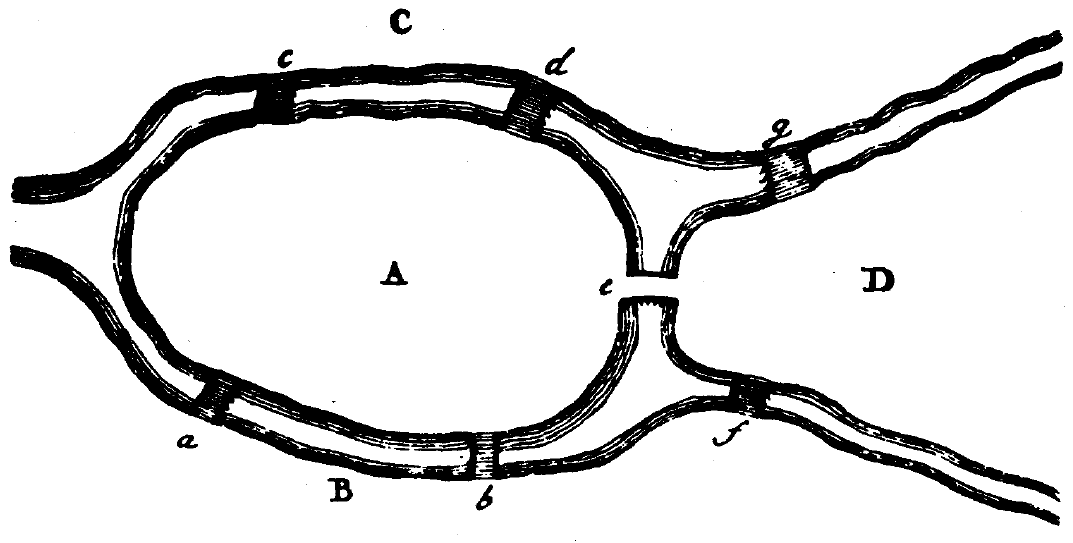
\includegraphics[width=\textwidth]{images/konigsberg.png}
		\subcaption{Rappresentazione dei ponti come descritta da Eulero.}
	\end{subfigure}
	\begin{subfigure}[b]{0.45\textwidth}
		\centering
		\begin{tikzpicture}
			\node[shape=circle,inner sep=2pt,draw,thick] (A) {A};
			\node[shape=circle,inner sep=2pt,draw,thick, below=of A] (B) {B};
			\node[shape=circle,inner sep=2pt,draw,thick, above=of A] (C) {C};
			\node[shape=circle,inner sep=2pt,draw,thick, right=of A] (D) {D};

			\draw[thick, bend left=10] (A) to (C);
			\draw[thick, bend right=10] (A) to (C);
			\draw[thick, bend left=10]  (A) to (B);
			\draw[thick, bend right=10] (A) to (B);
			\draw[thick]  (A) to (D);
			\draw[thick, bend left=10]  (C) to (D);
			\draw[thick, bend right=10]  (B) to (D);
		\end{tikzpicture}
		\subcaption{Rappresentazione come multigrafo.}
	\end{subfigure}
	\caption{I ponti di K\"onisberg.}
	\label{fig:ponti_konigsberg}
\end{figure}

Un antico problema chiedeva: è possibile partire da un punto qualsiasi della
città e attraversare tutti i ponti esattamente una ed una sola volta?
Per studiare questo problema, Eulero pensò di trasformare questa mappa in un
grafo, dove i vertici rappresentano le zone $A$, $B$, $C$, $D$ e i lati
sono i sette ponti della città. I grafi fatti in questo modo sono chiamati, oggi,
\textit{multigrafi}, ossia grafi i cui lati non sono un insieme ma un \textit{multinsieme},
insiemi con ripetizioni distinte: formalmenti, sono rappresentati con una mappa
che associa agli elementi il numero di ripetizioni. In termini di teoria dei
grafi, il problema si traduce come segue: $G$ ha un circuito (o ciclo)  che
passi esattamente una volta per ogni lato, ossia un \textbf{circuito euleriano}?

La risposta, in questo caso specifico, è no.
\begin{theorem}\label{thm:circ_euleriano}
	Esiste un circuito euleriano se e solo se tutti i vertici di un
	grafo connesso hanno grado pari.
\end{theorem}

\begin{proof}
	$\impliedby$ (Se tutti i vertici di un grafo hanno grado pari, allora esiste un
	circuito euleriano.) Sia $G$ un grafo in cui tutti i vertici hanno grado  pari.
	Partendo da un vertice a caso e seguendo un cammino formato da lati non
	ancora scelti (ossia si tiene traccia di quelli già ``consumati''), non può
	accadere che ci sia un arco non ancora scelto per planare sul nodo ma non
	un altro per uscirne, poiché questo significherebbe che il grado di tale nodo
	sia dispari.

	In questa costruzione succede, ad un certo punto, che si torna su uno
	dei vertici già visitati. Anche in questa situazione deve esistere un arco
	che permette di uscire da tale vertice: si segue quindi il lato non ancora
	utilizzato e si continua il percorso. Prima o poi, con questo ragionamento,
	si tornerà al vertice dal quale si è partiti, e questo è l'unico modo
	per costruire un circuito, che non è detto che sia euleriano, poiché non
	è detto che visiti tutti i lati. Tuttavia, si può ricominciare la visita partendo
	da un lato non ancora visitato: siccome il grafo è connesso, ci sarà modo
	di ricongiungersi al circuito iniziale.

\end{proof}

\noindent
Definiamo, invece, \textbf{circuito hamiltoniano} un circuto che passa esattamente una volta su ogni
vertice del grafo.

Un lemma utile è il seguente:
\begin{lemma}[Handshaking lemma]\label{lem:handshaking}
	In ogni grafo, il numero di vertici di grado dispari è pari.
\end{lemma}
\begin{proof}
	Deve essere
	$$
		\sum_{x \in V} d(x) = 2m
	$$
	ma la parità di una sommatoria dipende solo dai numeri dispari, infatti gli
	addendi pari non cambiano la parità. Se tale somma è pari, è necessario
	che il numero di addendi dispari sia pari.
\end{proof}


\noindent
Possiamo ora tornare al problema del commesso viaggiatore.

\popt {TravelingSalesman} {un grafo $G = (V,E)$ e un costo $\forall e \in E \delta_e$}
{Insieme ordinato di lati}
{Qual è il circuito hamiltoniano di minor costo?}
{Insieme ordinato di lati che formi un circuito hamiltoniano}
{$Min$}
{$\sum_{e \in \pi} \delta_e$}

\subsection{Algoritmo di Christofides}
\subsubsection{TSP su clique}
Si noti che non è necessario che esistano delle soluzioni ammissibili!
Per facilitare l'analisi e ottenere risultati migliori specializzeremo il problema in un certo modo:
analizzeremo il TSP su \textit{clique} (cricche), ossia un grafo
$G = (V, {V \choose{2}})$.

In quanto non è necessariamente vero che il grafo sia una cricca,
supponiamo di avere un grafo pesato non completo: lo trasformiamo in un
grafo completo
$$
	G = (V, E), \delta_e ~~ \leadsto ~~ K = (V, {V \choose 2}), \bar{\delta_e}
$$
definendo
$$
	\bar{\delta_e} =
	\begin{cases}
		\delta_e                    & e \in E    \\
		1 + \sum_{e \in E} \delta_e & e \notin E
	\end{cases}
$$
Se si trova una soluzione per $K$ che non utilizza nessun lato fittizio,
chiaramente tale soluzione è valida anche per $G$ ed è anche ottima, poiché
nessun circuito hamiltoniano può costare più di anche solo un lato fittizio.
In altre parole, la soluzione ottima coinvolge un lato fittizio se e solo se
per $K$ non vi sono soluzioni ammissibili.

\subsubsection{TSP metrico su clique}
Tuttavia, anche sulle clique il TSP è un problema estremamente complesso da
risolvere e, in generale, non è approssimabile a meno di una costante.
Con un ulteriore rilassamento riusciremo ad approssimare TSP, ossia
imponendo che le distanze formino una \textit{metrica} su $G$:
richiediamo che $G$ sia una cricca e $\delta_e$ sia una metrica, ossia $$
	\delta_{ij} \leq \delta_{ik} + \delta_{kj}
$$
% PROBLEMA: Se si crea il grafo completo utilizzando la costruzione precedente, la distanza 
% non è più una metrica..
Prima di designare l'algoritmo risolvente, introduciamo brevemente due problemi che
saranno utili.
\subsubsection{Minimo albero ricoprente}
\popt {MinimumSpanningTree} {$G = (V,E)$ \textit{bipartito}} {Insieme di lati}
{Qual è l'insieme di archi che copre i vertici con un costo minore?}
{L'insieme di lati è un albero, ossia un grafo connesso e aciclico}
{$Min$}{Cardinalità dell'insieme di lati}

Questo problema è risolvibile esattamente dall'algoritmo di Kruskal in tempo  $O(m\log(n))$.

\subsubsection{Matching perfetto a costo minimo}

\popt {MinimumWeightPerfectMatching} {$G = (V,E)$ con un numero pari di vertici}
{Insieme di lati}
{Esiste un matching perfetto?}
{Insieme di lati che formano un matching, ossia nessun vertice compare più di una volta, perfetto,
	ossia in cui compaiono tutti i vertici}
{$Min$}{Somma dei pesi degli archi scelti}

Anche questo problema è risolvibile in tempo polinomiale: un algoritmo famoso è
l'algoritmo \textit{dell'infiorescenza} che ha complessità $O(m \log(n))$.

\noindent
Possiamo ora passare all'algoritmo per risolvere istanze di \textsc{TravelingSalesman} su grafi
completi dotati di una distanza metrica.
\begin{algorithm}
	\caption{\textsc{ChristofidesTSP}}
	\KwInput{grafo $G = (V, {V \choose 2})$ con pesi $\delta_e$ che formano una metrica}

	$T = FindMST(G)$

	\tcc{$D$ è l'insieme dei vertici di grado dispari nel minimo albero ricoprente $T$. Per il
		\cref{lem:handshaking}, è $|D| \mod 2 = 0$.}
	$D = FindOddDegreeVertices(T)$

	\tcc{$G[D]$ è il grafo ristretto sui nodi di $D$}
	$G[D] = G(V \cap D, \cdots)$

	$M = FindPerfectMatching(G[D])$

	\tcc{\`E possibile che lo stesso lato appaia due volte, rendendo $H$ un multigrafo. Tutti i vertici
		in $H$ hanno grado pari, poiche' quelli che in $D$ hanno grado dispari hanno un nuovo lato.}
	$ H = T \cup M$

	$\pi = FindEulerianWalk(H)$

	$R = FindRepeatingVertices(\pi)$

	\For{$v : R$}
	{
		\tcc{per ogni vertice $v$ ripetuto nel cammino si cancellano due lati (uno entrante e uno uscente) e,
			siccome il grafo è una cricca, si inserisce un nuovo lato che collega i due vertici disconnessi
			(quello che portava a $v$ e quello raggiunto da $v$)}
		$\pi = RemoveAndReplace(\pi, v)$
	}

	\Return{$\pi$}
\end{algorithm}

\begin{lemma}\label{lem:tsp_T_leq_delta}
	Il costo dell'albero $T$ su $G$ è minore o uguale del costo ottimale del cammino hamiltoniano su $G$ metrico
	e completo:
	$$
		\delta(T) \leq \delta^*
	$$
\end{lemma}

\begin{proof}
	Sia $\pi^*$ un circuito hamiltoniano ottimo. Sia $e$ un qualunque lato che compare in $\pi^*$ e si
	consideri $\pi^* \setminus e$: il risultato è uno spanning tree (possibilmente minimo). Pertanto,
	$$
		\delta(T) \leq \delta(\pi^* \setminus e) \leq \delta^*
	$$
	poiché $T$ è \textit{un} minimo albero ricoprente.
\end{proof}
\begin{lemma}\label{lem:tsp_M_leq_hdelta}
	$$
		\delta(M) \leq \frac{1}{2}\delta^*
	$$
\end{lemma}
\begin{proof}
	Sia $\pi^*$ un circuito hamiltoniano ottimo.
	Dal \cref{lem:handshaking} sappiamo che un numero pari di vertici appare in $D$ come costruito
	nell'algoritmo: sia quindi $\pi'$ un qualunque circuito sui vertici di $D$.
	Questo circuito $\pi'$ attraverserà un numero minore o uguale di vertici attraversati da $\pi^*$,
	per ogni vertice in meno che deve attraversare dunque, invece di avere un lato che lo raggiunge
	ed uno da cui esce, ci sarà un solo lato che lo salta.
	Essendo $\delta$ una metrica dunque "saltare" un vertice dovrà costare per forza meno di prenderlo,
	quindi
	$$
		\delta(\pi') \leq \delta(\pi^*)
	$$
	Dividiamo i lati di $\pi'$ in due insiemi $M_1$ e $M_2$, in modo che si
	alternino nel cammino: essi sono due perfect matching su $D$. Allora
	\begin{align*}
		 & \delta(M_1) \geq \delta(M) \land \delta(M_2) \geq \delta(M)                      \\
		 & \implies \delta^* \geq \delta(\pi') = \delta(M_1) + \delta(M_2) \geq 2 \delta(M)
	\end{align*}
\end{proof}
\begin{theorem}
	L'algoritmo di Christofides è una $\frac{3}{2}$-approssimazione per il problema del
	commesso viaggiatore su grafi completi con distanza metrica.
\end{theorem}
\begin{proof}
	Siano $\tilde{\pi}$ il cammino hamiltoniano e $\pi$ il cammino euleriano costruiti dall'algoritmo.
	Allora deve essere $\delta(\tilde{\pi}) \leq \delta(\pi)$: $\pi$ passa per tutti
	gli archi di $H$ esattamente una volta:

	\begin{align*}
		 & \delta(\pi) = \sum_{e \in H} \delta(e)  = \delta(M) + \delta(T) \leq
		\underbrace{\frac{1}{2} \delta^*}_{\cref{lem:tsp_M_leq_hdelta}} +
		\underbrace{\delta^*}_{\cref{lem:tsp_T_leq_delta}}  = \frac{3}{2} \delta^*
	\end{align*}
\end{proof}

\begin{theorem}
	L'analisi di approssimazione  di TSP metrico su clique con Christofides è stretta.
\end{theorem}
\begin{proof}
	Dato $n$ pari ed $\epsilon \in (0,1)$, esibiamo il seguente grafo:

	\begin{figure}[h]
		\centering
		\begin{tikzpicture}
			\node[minimum size=15pt, draw, circle] (1) {$v_1$};
			\node[minimum size=15pt, draw, circle, right =of 1] (2) {$v_2$};
			\node[minimum size=15pt, draw, circle, right =of 2] (3) {$v_3$};
			\node[minimum size=15pt, draw, circle, right =of 3] (4) {$v_4$};
			\node[minimum size=15pt, draw, circle, right =of 4] (5) {$v_{n-2}$};
			\node[minimum size=15pt, draw, circle, right =of 5] (6) {$v_{n-1}$};
			\node[minimum size=15pt, draw, circle, right =of 6] (7) {$v_{n}$};

			\draw[] (1) to node [auto] {$1$} (2);
			\draw[bend right=35] (1) to node [below] {$1 + \epsilon$} (3);

			\draw[] (2) to node [auto] {$1$} (3);
			\draw[bend left=35] (2) to node [auto] {$1+\epsilon$} (4);

			\draw[] (3) to node [auto] {$1$} (4);
			\draw[bend right=30] (3) edge node [below] {$1 + \epsilon$}(5.5,-1);

			\draw[dotted] (4) to (5);

			\draw[] (5) to node [auto] {$1$} (6);
			\draw[bend left=35] (5) to node [auto] {$1+\epsilon$} (7);

			\draw[] (6) to node [auto] {$1$} (7);

			\draw[bend left=30] (6) edge node [auto] {$1 + \epsilon$} (7.5,-1);

		\end{tikzpicture}
	\end{figure}
	Tutti i lati mancanti hanno costo pari al costo del cammino minimo tra i due vertici del lato.
	L'algoritmo di Christofides seleziona il \textsc{MinimumSpanningTree} $T$, ossia il cammino composto da
	lati di costo $1$, quindi $\delta(T) = n - 1$. I nodi di grado dispari in $T$ sono
	i due estremi, quindi $D = \{v_1, v_n\}$. Il cammino minimo che li collega è
	un singolo lato che ha peso $\delta(M) = (1 + \epsilon) \frac{n}{2} + 1$.

	Al termine dell'algoritmo, il costo del circuito hamiltoniano ottenuto è
	$$
		\delta = n - 1 +  (1 + \epsilon) \frac{n}{2} + 1 = \frac{3}{2}n + \frac{\epsilon n}{2}
	$$
	Il costo del cammino ottimo è
	$$
		\delta^* = (1 + \epsilon) \frac{n}{2} + (1 + \epsilon) \frac{n}{2} +2 = (1 + \epsilon) n + 2
	$$
	quindi
	$$
		\frac{\delta}{\delta^*} = \frac{\frac{3}{2}n + \frac{\epsilon n}{2}}{(1 + \epsilon)n +2}
		= \frac{\frac{3}{2} n + \frac{n}{2}\epsilon}{n + 2 + \epsilon n} = \frac{3}{2}
	$$
	per $n \rightarrow \infty$ e $\epsilon \rightarrow 0$.
\end{proof}

% lezione 9 - 27/10/2021
\subsection{Inapprossimabilità di TSP}
La situazione non è altrettanto positiva per il caso generale del TSP:
\begin{theorem}
	Decidere se un grafo contiene un cammino hamiltoniano è un problema in $\mathbf{NP-completi}$.
\end{theorem}

\begin{theorem}
	Non esiste alcun $\alpha$ tale che \textsc{TravelingSalesman} sia $\alpha$-approssimabile a meno che
	$\mathbf{P} \neq \mathbf{NP}$.
\end{theorem}
\begin{proof}
	(per assurdo.)
	Sia $G = (V,E)$ un grafo che si completa creando $G'$: su questo grafo definiamo
	una nozione di distanza
	$$
		d(x,y) =
		\begin{cases}
			1                         & x, y \in E    \\
			\lceil \alpha n \rceil +1 & x, y \notin E
		\end{cases}
	$$
	Se $G$ ammette un circuito hamiltoniano, in $G'$ quel circuito ha costo
	$n$, poiché tocca tutti i vertici concludendo il circuito. Se $G$ non ammette
	un circuito hamiltoniano su di esso, possiamo concludere che in $G'$ tutti i
	circuiti hamiltoniani passano per almeno un lato di costo $\lceil \alpha n \rceil +1 $,
	quindi il circuito del costo hamiltoniano minimo è almeno $\lceil \alpha n \rceil + 1$.
	Se $G$ ha un circuito hamiltoniano l'algoritmo $\alpha$ approssimante per
	trovare cammini hamiltoniani in $G'$ (che, per assurdo, assumiamo esistere),
	troverà un circuito di costo minore o uguale a $\alpha n$ (poiché è $\alpha$-approssimante);
	se $G$ non ammette un circuito hamiltoniano, troverà un circuito di costo
	maggiore di $\lceil \alpha n \rceil +1$.
	\`E impossibile che $\alpha < \lceil \alpha n \rceil + 1$, altrimenti sapremmo
	decidere se $G$ ammette circuiti hamiltoniani. Ossia, deve essere
	$$
		\alpha > \frac{\lceil \alpha n \rceil + 1}{n} \geq \frac{\alpha n +1}{n} = \alpha + \frac{1}{n}
	$$
	ossia $\alpha \geq \alpha + \frac{1}{n}$, impossibile.
	Concludiamo che \textsc{TravelingSalesman} $\notin \mathbf{APX}$.
\end{proof}

\section{Problema del 2-carico}
In \textsc{LoadBalancing}, l'input era composto da  $t_0, t_1, \cdots, t_{n-1} \in \mathbb{N}^+$
tasks e un numero $m$ di macchine. L'obiettivo era costruire degli assegnamenti
tali per cui il carico massimo di una macchina è il minimo possibile. La versione
\textsc{$2$-LoadBalancing} è una specializzazione in cui $m = 2$.

\subsection{Algoritmo PTAS}
Due algoritmi per risolvere \textsc{LoadBalancing} sono stati proposti: greedy
(\cref{algo:greedybalance}) o con ordinamento iniziale delle task
(\cref{algo:sortedbalance}).
Ora, faremo molto meglio descrivendo un algoritmo che porta \textsc{$2$-LoadBalancing} in $\mathbf{PTAS}$:
daremo quindi un tasso di approssimazione vincolante per la soluzione trovata -
tuttavia l'algoritmo risulterà esponenziale in tale tasso.

\begin{algorithm}[h]
	\caption{PartitionBalance}
	\label{algo:partitionbalance}
	\KwInput{$m_1, m_2, t_0, ..., t_{n-1}, \epsilon$}

	\If {$\epsilon \geq 1$}
	{
		$m_1.tasks = \{t_0, \cdots, t_{n-1}\}$

		\Return
	}

	$tasks = [t_0,\cdots, t_{n-1}].nonDecreasingSort()$

	$k = \lceil \frac{1}{\epsilon} -1 \rceil$

	\tcc{Esegui l'algoritmo esaustivo sui primi $k$ task}
	$optPartition = findOptimalPartition(tasks[0\cdots k-1])$

	$GreedyBalance(m_1, m_2, tasks[k\cdots])$

\end{algorithm}

\begin{theorem}
	L'\cref{algo:partitionbalance} è polinomiale in $n$ (ma non in $\epsilon$) e
	produce una $1+ \epsilon$ approssimazione per \textsc{$2$-LoadBalancing}.
\end{theorem}

\begin{proof}
	Se $\epsilon \geq 1$, assegnare tutte le task ad una sola macchina non può
	essere peggio del doppio del costo ottimale.
	Altrimenti, proseguiamo seguendo l'esecuzione dell'algoritmo.
	I primi $k$ task vengono assegnati in modo ottimale. I seguenti $n - k$ task
	vengono assegnati in maniera greedy. Assumiamo, senza perdita di generalità,
	che $w(m_1) \geq w(m_2)$. Sia $h$ l'indice dell'ultimo task assegnato alla
	macchina $m_1$. Abbiamo due casi:
	\begin{itemize}
		\item $h < k$. Tutti i task assegnati in maniera greedy appartengono alla
		      macchina $m_2$. Siccome i task assegnati a $m_1$ sono assegnati in
		      modo ottimale, il costo massimo $w(m_1)$ è ottimale.
		\item $h \geq k$. Dopo la fase ottima la macchina $m_1$ riceve altri task.
		      Sia $L = \frac{\sum_{i} t_i}{2}$, facciamo due osservazioni che ci 
			  torneranno utili:
		      \begin{align*}
			       & w(m_1) - t_h  \leq w(m_2) \text{ nel momento in cui si assegna } h \leq w(m_2)                        \\
			       & \implies 2*w(m1) - t_h \leq w(m_1) + w(m_2) = 2L                                                      \\
			       & \implies w(m_1) - \frac{t_h}{2} \leq L
			  \end{align*}
			  e
			  \begin{align*}
				   & 2L  = t_0 + t_1 + \cdots + t_k + t_h + \cdots + t_{n-1} \geq t_h (k+1)                                \\
			  \end{align*}
			  Ora consideriamo il rapporto tra il valore restituito dall'algoritmo,
			  cioè il carico della macchina più carica (dunque $w(m_1)$). Ricordiamo che
			  $w^* \geq L$
			  \begin{align*}
				   & \frac{w}{w^*} = \frac{w(m_1)}{w^*} \leq \frac{w(m_1)}{L} \leq                                         \\
				   & \leq \frac{\frac{t_h}{2}+L}{L} = 1 + \frac{t_h}{2L} \leq & \text{per la prima osservazione}           \\
				   & \leq 1 + \frac{t_h}{2 \frac{t_h}{2} \cdot (k + 1)} = 1 + \frac{1}{1 + k} & \text{per la seconda osservazione} \\
		      \end{align*}
		      Ma $k = \lceil \frac{1}{\epsilon}\rceil - 1 \geq \frac{1}{\epsilon} - 1$, quindi:
		      \begin{align*}
				   & 1 + \frac{1}{1 + k} \leq 1 + \frac{1}{1 + \frac{1}{\epsilon} - 1} = 1 + \epsilon
		      \end{align*}
	\end{itemize}
\end{proof}

\begin{theorem}
	L'algoritmo ha tempo d'esecuzione $O(n\log{n} + 2^{\frac{1}{\epsilon}})$.
\end{theorem}
\begin{corollario}
	Essendo uguale a \textsc{2-LoadBalancing},  \textsc{MinimumPartition} $\in \mathbf{PTAS}$.
\end{corollario}

\section{Problema dello zaino}
\popt {Knapsack} {$n$ oggetti con valori $v_0, \cdots, v_{n-1} \in \mathbb{N}$ e
	pesi $w_0, \cdots, w_{n-1} \in \mathbb{N}$ e una capacità $W \in \mathbb{N}$} {Insieme di oggetti $S$}
{Qual è l'insieme di oggetti di valore maggiore che si può scegliere senza eccedere
	la capacità $W$?}
{Scelta di oggetti che non eccedono $W$: $\sum_{i \in S} w_i \leq W$}
{$Max$}{Valore degli oggetti in $S$: $\sum_{i \in S} v_i$}

\begin{theorem}
	\textsc{KnapsackProblem} $\in \mathbf{NPO-completi}$.
\end{theorem}

\subsection{Algoritmo esponenziale basato su programmazione dinamica}
Come solitamente accade quando si desidera trovare un algoritmo basato
sulla \textit{programmazione dinamica}, suddividiamo il problema in problemi
più piccoli: costruiamo una matrice
$$
	vOPT[i, w] =  \text{ massimo valore di } i \text{ oggetti con zaino di capacità } w
$$
con $ i \leq n$ e $w \leq W$. Ovviamente, ciò che ci interessa è $vOPT[n, W]$,
ossia il valore massimo ottenibile considerando tutti gli $n$ oggetti
e con capacità $W$.
In quanto il valore ottenibile scegliendo $0$ oggetti è $0$, abbiamo che, per qualsiasi
capacità, $vOPT[0, \_] = 0$ - analogamente, siccome nessun oggetto può essere scelto
se la capacità è $0$, deve essere $vOPT[\_, 0]  = 0$.

L'entry della $i+1$-esima riga nella $w+1$-esima colonna
si costruisce decidendo se inserire o meno l'$i$-esimo oggetto:
$$
	vOPT[i+1, w] =
	\begin{cases}
		vOPT[i, w]             & w_i > w    \\
		vOPT[i, w - w_i] + v_i & w_i \leq w
	\end{cases}
$$

Questo algoritmo, ovviamente, non può essere polinomiale (altrimenti sarebbe
$\mathbf{P} = \mathbf{NP}$) -- è vero che il
numero di entry nella matrice è $n \cdot w$, ma l'algoritmo non è polinomiale nella
lunghezza binaria dell'input $W$, bensì è esponenziale, rendendo quindi l'algoritmo
\textit{pseudopolinomiale}.

\subsection{Algoritmo FPTAS basato su programmazione dinamica}
Per cercare di ovviare al problema della pseudopolinomialità del metodo precedente,
scomponiamo il problema in termini di oggetti e valore (invece che peso):
$$
	wOPT[i, v] = \text{minimo peso necessario per i primi } i \text{ oggetti con valore } \geq v
$$
In $wOPT$ le colonne rappresentano valori tra $[0, \sum_{i}v_i]$ - in realtà,
approssimiamo questo range con $[0, n\cdot v_{max}]$, con $v_{max} = \max_i v_i$.

Sull'ultima riga troveremo il minimo peso necessario per scegliere $n$ oggetti;
potrà accadere che per molte colonne $wOPT[i,v] > W$, che rappresentanos
soluzioni non accettabilil; dovremo quindi cercare la prima entry che non sfora
la capacità $W$. La prima colonna sarà $wOPT[\_,0] = 0$, mentre, inizialmente,
si imposta $wOPT[0,\geq1] = \infty$.

La regola di riempimento che definiamo è
$$
	wOPT[i+1, v] = \min(wOPT[i, v], wOPT[i, \max(v-v_i, 0)] + w_i)
$$

Benché apparentemente sembra non ci sia alcun vantaggio, in questo frangente
possiamo operare delle modifiche sulla matrice: l'idea è quella di ``schiacciare''
le colonne, operando una divisione o un cambio di misura, nonostante venga
in questo modo introdotta un'approssimazione dei valori. Introduciamo,
quindi, un \textit{valore di scala}:
$$
	\theta = \frac{\epsilon v_{max}}{2n}
$$
e l'obiettivo finale sarà avere una $1+\epsilon$-approssimazione.
Sia quindi $X=(v_i, w_i, W)$ l'input del problema; siano

$$
	\bar{v_i} = \lceil\frac{v_i}{\theta}\rceil\cdot \theta, ~~ \hat{v_i} = \lceil \frac{v_i}{\theta}\rceil
$$
ai quali associamo i relativi problemi $\bar{X} = (\bar{v_i}, w_i, W)$
e $\hat{X} = (\hat{v_i}, w_i, W)$
che avranno delle soluzioni ottime $v^*, \bar{v}^*$ e $\hat{v}^*$, derivanti
da insiemi $S^*, \bar{S}^*$ e $\hat{S}^*$.

\begin{oss} \label{oss:knapsack_barv_t_hatv}
	Banalmente,
	$$
		\bar{v}^* = \theta \hat{v}^*
	$$
	In altre parole, risolvere $\hat{X}$ o risolvere $\bar{X}$ restituisce le
	stesse soluzioni, pertanto
	$$
		\bar{S}^* = \hat{S}^*
	$$

\end{oss}

\begin{lemma}
	Sia S una soluzione ammissibile per il problema. Allora
	$$
		(1+\epsilon)\sum_{i \in \hat{S}^*} v_i \geq \sum_{i \in \bar{S}^*} v_i
	$$
\end{lemma}
\begin{proof}
	\begin{align*}
		 & \sum_{i \in S} v_i \leq \sum_{i \in S} \bar{v}_i  \text{ grazie all'arrotondamento per eccesso}                      \\
		 & \leq \sum_{ i \in \bar{S}^*} \bar{v}_i  \text{ poiché è la soluzione ottima}                                         \\
		 & = \sum_{ i \in \hat{S}^*} \bar{v}_i \text{ poiché } \hat{S}^* = \bar{S}^* \text{ da \cref{oss:knapsack_barv_t_hatv}} \\
		 & = \sum_{i \in \bar{S}^*} \bar{v}_i \leq \sum_{i \in \hat{S}^*} (v_i + v) \leq
		\sum_{i \in \hat{S}^*} v_i + n \theta = \sum_{i \in \hat{S}^*} v_i + n \frac{\epsilon v_{max}}{2 n}
	\end{align*}
	quindi
	$$
		\sum_{i \in S} v_i  \leq \sum_{i \in \hat{S}^*} v_i + \frac{\epsilon v_{max}}{2}
	$$

	In particolare, questo vale per la soluzione composta
	solamente dall'oggetto con valore massimo $S = \{max\}$, da cui segue
	\begin{align*}
		 & v_{max} \leq \sum_{i \in \hat{S}^*} v_i + \frac{\epsilon v_{max}}{2}
		\leq \sum_{i \in \hat{S}^*} v_i + \frac{v_{max}}{2} \text{ poiché } \epsilon \leq 1         \\
		 & \implies \sum_{i \in \hat{S}^*} v_i \geq \frac{v_{max}}{2}                               \\
		 & \implies \sum_{i \in S} v_i \leq \sum_{i \in \hat{S}^*} v_i + \frac{\epsilon v_{max}}{2}
		\leq \sum_{i \in \hat{S}^*}v_i + \epsilon \sum_{i \in \hat{S}^*} v_i = (1 + \epsilon) \sum_{i \in \hat{S}^*} v_i
	\end{align*}
\end{proof}
\begin{theorem}
	$$
		(1+\epsilon)\sum_{i \in \hat{S}^*} v_i \geq \sum_{i \in S^*} v_i = v^*
	$$
	Risolvendo il problema $\hat{X}$ si ottiene una soluzione il cui valore
	per il problema originale è
	$\frac{1}{1+\epsilon}$
	volte l'ottimo.
\end{theorem}

\begin{algorithm}
	\caption{FPTASKnapsack}
	\label{algo:FPTASKnapsack}
	\KwInput{$X = (v_i, w_i, W), \epsilon$}

	$
		\hat{X} = getFrom(X, \epsilon)
	$

	\tcc*{La soluzione così trovata è una $(1 + \epsilon)-$approssimazione}

	\Return {$solveWithWOpt(\hat{X})$}
\end{algorithm}

Dobbiamo ora convincerci che \cref{algo:FPTASKnapsack} termini
in tempo polinomiale: l'ultima colonna sarà $n \hat{v}_{max}$;
sappiamo che
$$
	v_{max} = \lceil \frac{v_{max}}{\theta} \rceil = \lceil \frac{v_{max} n}{\epsilon v_{max}} \rceil
	=\lceil \frac{n}{\epsilon}\rceil
$$
pertanto il numero di colonne
$$
	n\hat{v}_{max} \leq \frac{n^2}{\epsilon} + n
$$
polinomiale nell'input e in $\epsilon$.




%%% Local Variables:
%%% TeX-master: "../main"
%%% End:
